\documentclass{report}
\usepackage[utf8]{inputenc}
\usepackage[toc,page]{appendix}
\usepackage[letterpaper, margin=1in]{geometry}
\usepackage{tocbibind}
\usepackage{datetime}
\usepackage{multicol}
\usepackage{graphicx}
\usepackage{subcaption}
\usepackage{float}
\usepackage{siunitx}
\usepackage{amsmath}
\usepackage{booktabs}
\usepackage{makecell}
\usepackage{hyperref}

\author{Waterloop Team}

\setlength{\parindent}{0pt}
\setcounter{secnumdepth}{5}
\setcounter{tocdepth}{5}
\title{Waterloop Final Design Package}

\newdate{date}{05}{01}{2018}
\date{\displaydate{date}}

\renewcommand{\contentsname}{Table of Contents}
\let\oldparagraph\paragraph

\renewcommand{\paragraph}[1]{\oldparagraph{#1}\mbox{}\\}

\begin{document}
    \maketitle
    Revised \displaydate{date}\\
    
    Prepared by the Waterloop Team.
    
    Prepared for Space Exploration Technologies Corp. for the Hyperloop Pod Competition.\\
    
    \copyright \ 2017 by Waterloop.
    
    All rights reserved. Not for public distribution.\\
    
    Document approved for submission by the Waterloop executive team on \_\_\_.
    
    \tableofcontents
    \newpage
    
    \chapter*{Quick Reference}
    \begin{enumerate}
        \item Description of team and updated list of all associated team members and advisors
        \item Design description for Pod. At a minimum, this should include:
        \begin{enumerate}
            \item Pod top-level design summary
            \item Pod dimensions
            \item Pod mass by subsystem
            \item Pod payload capability
            \item Pod materials
            \item Pod power source and consumption
            \item Pod navigation mechanism
            \item Pod levitation mechanism (if any)
            \item Pod propulsion mechanism
            \item Pod braking mechanism
            \item Pod stability mechanisms (e.g. attitude and lateral motion)
            \item Pod aerodynamic coefficients
            \item Pod magnetic parameters (if applicable)
        \end{enumerate}
        \item Predicted Pod thermal profile
        \item Predicted Pod trajectory (speed versus distance)
        \item Predicted vibration environments
        \item Pod structural design cases: at a minimum, this shall include initial acceleration, nominal deceleration, and a reasonably foreseeable off-nominal crash
        \item Pod production schedule
        \item Pod cost breakdown
        \item Sensor list and location map
        \item Comments on scalability to an operational Hyperloop with respect to:
        \begin{enumerate}
            \item System size (increased tube length, tube diameter, and Pod size)
            \item Cost (both production and maintenance)
            \item Estimated Pod mass and cost if built full-scale
            \item Maintenance (e.g. not requiring specialized alignment tools, hot-swappable subsystems)
        \end{enumerate}
        \item Loading and unloading plan
        \begin{enumerate}
            \item Full descriptions of all functional tests (see Sections 10 and 12)
            \item Full description of Ready-to-Launch checklist/state (e.g. Loop Computer in “Launch Mode” and sending telemetry, Pod hovering at 0.25 inches)
            \item Full description of Ready-to-Remove checklist/state (e.g. Wheels locked, Power Off)
            \item Description of how Pod is moved from Staging Area to Hyperloop
            \item Description of how Pod is moved from Hyperloop to Exit Area
        \end{enumerate}
        \item List and description of any stored energy on the Pod (i.e. pressure vessels, batteries)
        \item List of any hazardous materials, if any
        \item Description of safety features including:
        \begin{enumerate}
            \item Hardware and software inhibits on braking during the acceleration phase
            \item Mechanisms to mitigate a complete loss of Pod power
            \item Pod robustness to a tube breach resulting in rapid pressurization
            \item Fault tolerance of braking, levitation, and other subsystems
            \item Single point of failures within the Pod
            \item Recovery plan if Pod becomes immovable within tube
            \item Implementation of the Pod-Stop command
        \end{enumerate}
        \item Component and system test program before the Pod arrives for the Competition
        \item Vacuum Compatibility Analysis
        \item If a returning Pod, highlight the modifications and upgrades made
    \end{enumerate}
    
    \addcontentsline{toc}{chapter}{Quick Reference}
    
    \chapter{Introduction}
    
    \section{Our Team}
    We are Waterloop, a student design team … demographics…\\
    
    We are the only all-Canadian organization to have built a functioning Hyperloop prototype, and we intend to continue to represent Canadian innovation through participation in the 2018 Hyperloop Competition. [something something trudeau and gg]\\
    
    Our mission has several components:
    To strongly represent Waterloo as a hub for Canadian innovation through the SpaceX Hyperloop Competition.
    \begin{itemize}
        \item To teach technical skills, strong engineering practices, and teamwork.
        \item To reach out to inspire and cultivate young innovators from all backgrounds.
        \item To make possible a future that is worth building.
    \end{itemize}
    Who we are\\
    Mission\\
    Marketing, outreach, stats on how impactful we are - blogs and team member profiles, heforshe\\
    Brief mention of financials, convince them we can fund it
    
    \section{Team Member Directory}
    \begin{center}
        \textsf{Board of Advisors}
    \end{center}
    \begin{multicols}{2}
        \begin{center}
            Serhiy Yarusevych\\
            a\\
        \end{center}
        \columnbreak
        \begin{center}
            Victor Qian\\
            b
        \end{center}
    \end{multicols}
    \begin{center}
        \textsf{Team Leadership}
    \end{center}
    \begin{multicols}{4}
        \begin{center}
            Benjamin Tonita\\
            \begin{small}
                -Integration Engineer-\\
            \end{small}
        \end{center}
        \columnbreak    \begin{center}
            Clive Chan\\
            \begin{small}
                -Technical Director-\\
            \end{small}
        \end{center}
        \columnbreak    \begin{center}
            Jason Pan\\
            \begin{small}
                -Administrative Director-\\
            \end{small}
        \end{center}
        \columnbreak
        \begin{center}
            Jimmy Zhou\\
            \begin{small}
                -Integration Engineer-
            \end{small}
        \end{center}
    \end{multicols}
    \begin{center}
        \textsf{Team Members}\\
        \hfill\\
        \begin{tabular}{| c | c | c | c |}
            \hline
            &   &   & \\
            \hline
            &   &   & \\
            \hline
        \end{tabular}
    \end{center}
    \begin{itemize}
        \item Advisors: Serhiy Yarusevych, Victor Qian
        \item Directors: Jason Pan, Clive Chan
        \item Integration Engineers: Jimmy Zhou, Benjamin Tonita
        \item Administrative Leads: Nicholas Jelich, Natalia Zigante, Nafee Hasan, Aditya Arora
        \item Technical Leads: William Ngana, Deep Dhillon, Ruslan Nikolaevra, Urooj Khaleeli, Jimmy Zhou, Benjamin Tonita, Chawthri Kanagarasa
    \end{itemize}
    
    \section{Sponsors}
    Thanks to all our sponsors, past and present
    
    \begin{itemize}
        \item Which logos? Sponsorship team should decide
        \item We’ll have more soon
    \end{itemize}
    
    \section{Acknowledgements}
    
    \begin{itemize}
        \item Advisors: Serhiy, Victor
        \item Waterloo Formula Electric for guidance on embedded and electrical
        \item Sandra \& Sedra Student Design Centre
        \item Various other things
    \end{itemize}
    
    \chapter{Top-Level Design}
    Labeled CAD (Exploded? Semitransparent? Color coded?)\\
    
    Our pod design process for Competition III began with the goal of building the fastest possible pod. Based purely on specific power and energy of lithium ion batteries (and perhaps supercapacitors), it is theoretically possible to achieve speeds above Mach 1 within the 1-mile Hyperloop test track. Our pod this year is designed to achieve 100 m/s, and we are working gradually toward higher and higher speeds for future competitions.
    
    
    \section{Summary of design}
    Our pod consists of the following major components:
    \begin{itemize}
        \item Propulsion: Friction drive (wheels)
        \item Braking: High speed eddy current braking, low speed caliper brakes
        \item Lateral stability: Freely spinning wheels
        \item Frame: Aluminum ladder frame
        \item
    \end{itemize}
    Uniqueness/Novelty\\
    Changes from PDB and reasoning for changes\\
    If reusing a system in whole or part, explain changes\\
    
    \subsection{Size and Mass}
    The size of the pod is primarily dictated by the size of the propulsion system and the size of the I-beam.\\
    Table: pod dimensions, mass by subsystem\\
    Overall weight distribution/Center of mass\\
    The cross-section of the pod is small enough that aerodynamic effects like the Kantrowitz limit\\
    are negligible.\\
    
    \subsection{Energy Storage and Usage}
    Where is energy stored onboard the pod?
    \begin{itemize}
        \item Huge batteries
        \item Air tanks
        \item Lateral/EC Brakes springs?
    \end{itemize}
    Where is energy used onboard the pod?
    \begin{itemize}
        \item Friction drive
        \item Electronic systems (electrically isolated)
    \end{itemize}
    
    \subsection{Overall pod thermal profile}
    How are various parts of the pod cooled? (summarize)
    
    \subsection{Predicted Pod trajectory}
    Speed versus distance graph
    
    \section{Scalability}
    Our pod design is essentially the simplest possible design for a Hyperloop. However, it is difficult to scale to high-subsonic speeds.
    “gain experience with high power systems and high speed stability and braking systems.”\\
    
    Preliminary analysis on scalability to an operational Hyperloop with respect to:
    \begin{itemize}
        \item System size (increased tube length, tube diameter, and Pod size)
        \item Cost (both production and maintenance)
        \item Estimated Pod mass and cost if built full-scale
        \item Maintenance (e.g. not requiring specialized alignment tools, hot-swappable subsystems)
        \item Power, cooling, safety, etc.
        \item Propulsion effectiveness
    \end{itemize}
    
    
    \chapter{Subsystems}
    
    \section{Propulsion}
    Propulsion, the new challenge for Competition III, is the most challenging subsystem to design, and its design additionally dictates the design of every other component on the pod. To select the best possible method of propulsion given competition constraints, we conducted a series of preliminary analyses on possible propulsion designs, the most promising of which were the Friction Drive and Linear Induction Motor (LIM). We eventually chose to invest fully into the Friction Drive design, due to the complexity, mass, and cost of a LIM suited for competition accelerations. [2-3 SUMMARY SENTENCES ABOUT FRICTION]. Friction drive serves as a safe and reliable form of propulsion as it is well researched and tested in many different fields.
    
    \subsection{Propulsion Feasibility \& Design Candidates}
    We investigated several different methods of propulsion, including chemical propulsion, railgun propulsion, air pressure propulsion, and others. For safety, mass, and cost reasons, our most promising designs were friction drive and linear induction motor. Our initial design, submitted for the Preliminary Design Package, included a LIM.\\
    
    However, later calculations based on commercially available LIMs showed that off-the-shelf products would be abysmally unsuited for the Hyperloop competition; most such LIMs have a very narrow operating range of velocity, outside of which the motor becomes extremely inefficient. First-principles analysis based on [PAPERS?] showed some promise, but this would require a ground-up design of a variable-pitch linear induction motor, which seems to be on the current cutting edge of linear motor research.\\
    
    [some kind of diagram or numbers about this @Ben]\\
    
    We decided to table the LIM design, due to the relative inexperience of our team with electromagnetic propulsion, as well as the very high mass and cost. We do, however, plan to continue researching this to be ready for next year’s competition. Friction drive, though it does not scale well to Hyperloop speeds, will still allow us to gain experience with high power systems and high speed stability and braking systems.\\
    
    \subsection{Overall Design}
    Full labeled detailed CAD\\
    Mass, power, etc.\\
    Full cost breakdown, comments on manufacturability and production costs\\
    “A full Bill of Materials can be found in Appendix C.”
    
    \subsection{Structural}
    What are several reasonable and edge-case loading scenarios, and how does the FEA look for all of those? Justify your “reasonable” scenarios. If possible to simulate, how many cycles might it withstand?\\
    
    How will we deal with stability despite imperfections and irregularities in the track, and resulting modes of vibration? (Simulation would be good)
    
    \begin{figure}[H]
        \centering
        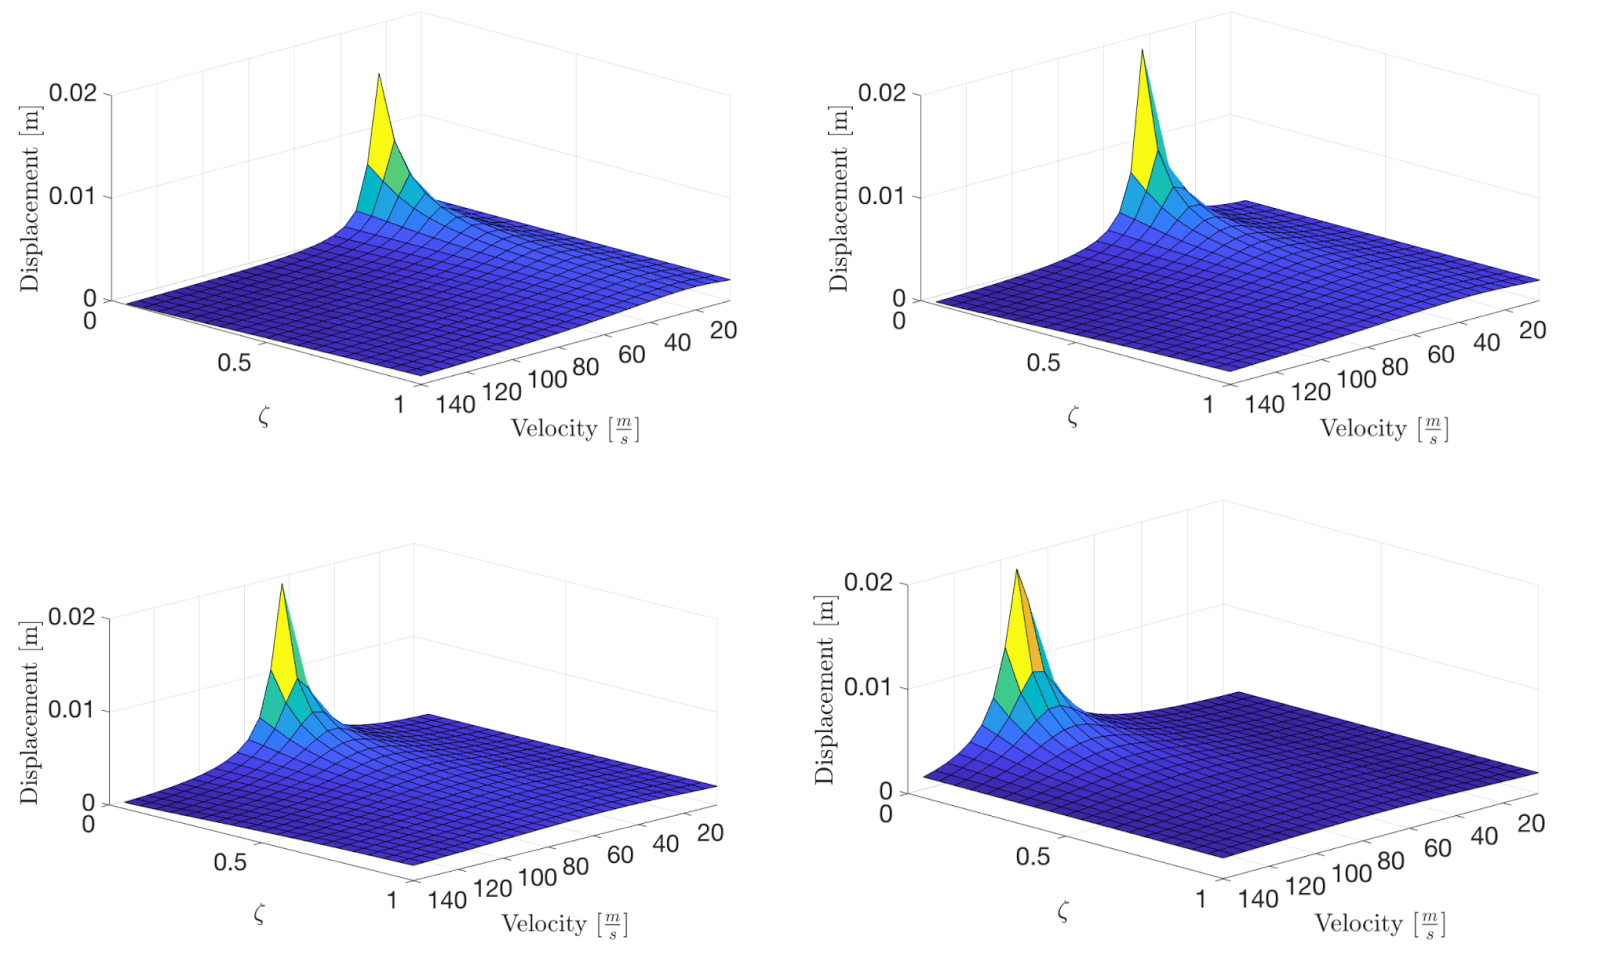
\includegraphics[width=\textwidth]{images/fig1}
        \caption{Spring constant of a. 100,000, b. 250,000, c. 500,000, and d. 1,000,000}
    \end{figure}
    
    \begin{figure}[H]
        \centering
        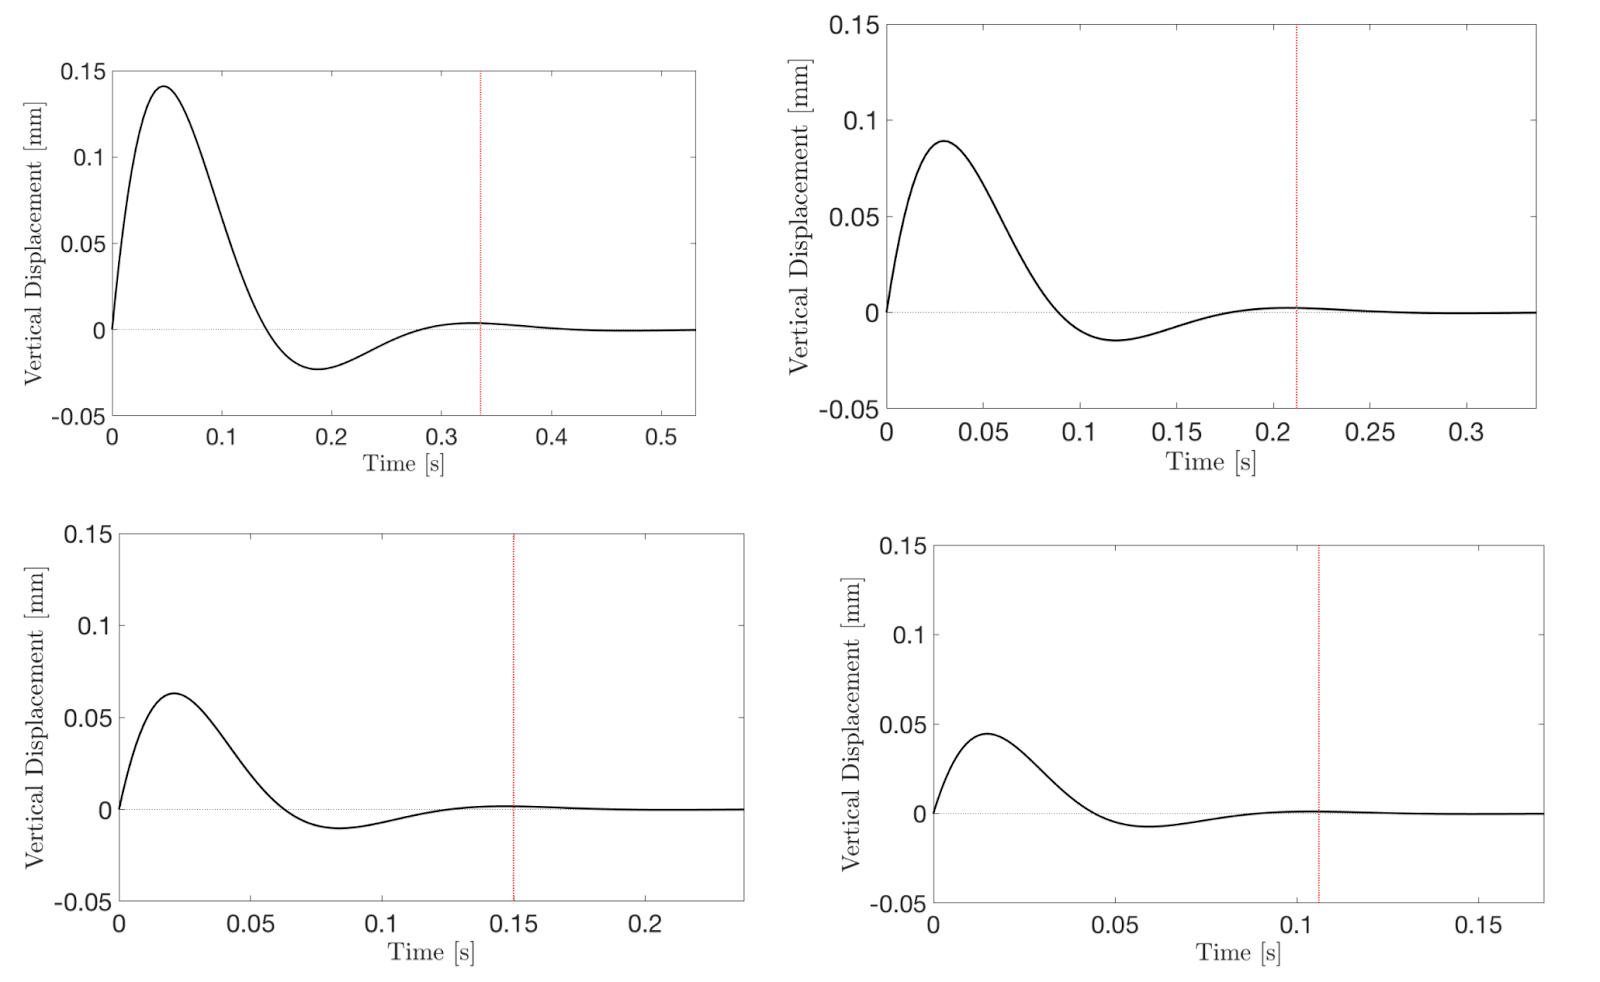
\includegraphics[width=\textwidth]{images/fig2}
        \caption{Spring constant of a. 100,000, b. 250,000, c. 500,000, and d. 1,000,000}
    \end{figure}
    We performed two separate vibrational analyses, in the vertical and horizontal directions, with two separate vibrational damping systems. Based on the construction of the track, the horizontal direction will likely be by far the most problematic; this analysis is detailed in the Lateral subsystem. The vertical damping system is closely integrated into the friction drive system, and so is described here.\\
    
    First, to determine design parameters of the springs and dampers, several simulations were performed. Different spring constants were chosen, and simulations for each were created using MatLab. The simulated pod was excited with a sinusoidal displacement, with amplitude as the maximum I-beam height tolerance and frequency matching the rate of I-beams passing by the pod. The magnitude of the maximum resulting pod displacement from the beam was plotted for each value of damping coefficient and speed (Figure 1). This series of plots shows the most dangerous combinations of damping coefficient and velocity. For each value of the spring coefficient, as the damping is increased, the vibrations become less intense. It was decided that a value of damping coefficient between [0.5 - 1.0] would be optimal in order to reduce pod vibrations.  Moving forward with this analysis, the response of the pod to a sudden displacement step was measured for a damping coefficient of 0.5 with varying spring constants. This is shown in figure ii. It can be seen that as the spring coefficient is increased, the pod returns to the initial position much faster, which is shown by the red line. Also, as the spring coefficient is increased, the maximum displacement also decreases. Therefore, it was decided that the spring coefficient and damping coefficient should have values of 500,000? And 0.5? Respectively.
    \begin{figure}[H]
        \centering
        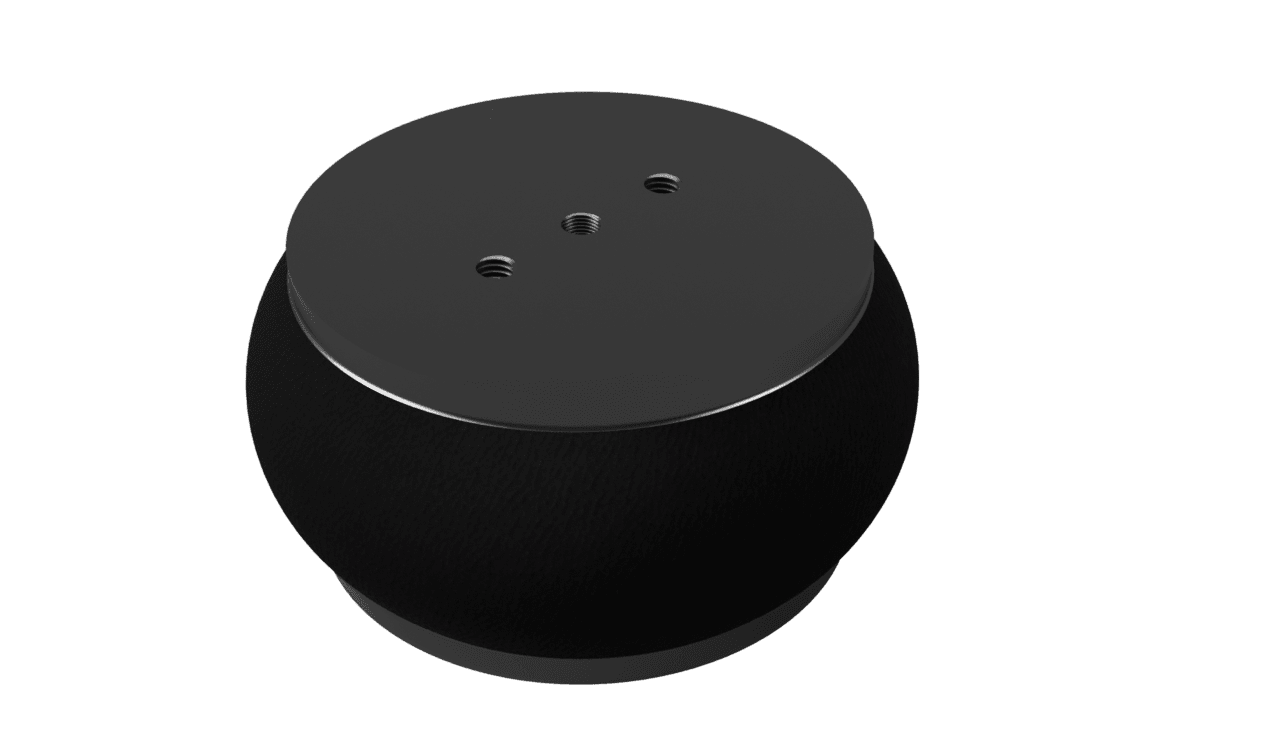
\includegraphics[width=\textwidth]{images/fig3}
        \caption{Caption needed}
    \end{figure}
    The motor-wheel assembly is mounted to the frame using airbag suspension and a Watts linkage. The motor and wheel are isolated from the frame as one unit to avoid the use of a belt tensioner, as the motor and wheel move in unison. Airbags were chosen for their easy adjustability via air pressure and their ability to take high loads.  A Watts linkage allows the unit to move in the normal axis relative to the frame while remaining secured in both the lateral and longitudinal axes.\\
    
    The material for structural members of the friction drive is Aluminum 6061-T6, chosen for its ease of machinability and high strength to weight ratio. The disadvantages of aluminum in its difficulty of welding was a non-issue, as the structure was not designed to have welded joints.\\
    
    Add FEA, explain forces and BC\\
    Maybe add properties of 6061? AZ did it\\
    There’s some calcs we can do with max tension / compression of those linkage rods\\
    
    Mention factors of safety for everything
    
    \subsection{Motor}
    Comments on why we selected the motor we did\\
    
    We investigated different types of electric motors to select one that was best suited for our applications, primarily AC induction motors and DC brushless motors. Specifically, axial flux motors were favoured due to their high power density and efficiency. These motors are very light and can provide high torque and power with low heat loss.\\
    
    It came to several choices of motors from electric motor manufacturers, YASA and EMRAX, that specialize in producing commercial axial flux motors. Several product criteria that affected this choice included:
    
    \begin{itemize}
        \item Specific power density
        \item RPM range
        \item Torque and power profiles
        \item Efficiency/Thermal Generation
        \item Mass
        \item Power consumption
        \item Cost
    \end{itemize}
    
    Based on these criteria, the EMRAX 268 was chosen.\\
    
    EMRAX 268 Specifications
    \begin{figure}[H]
        \centering
        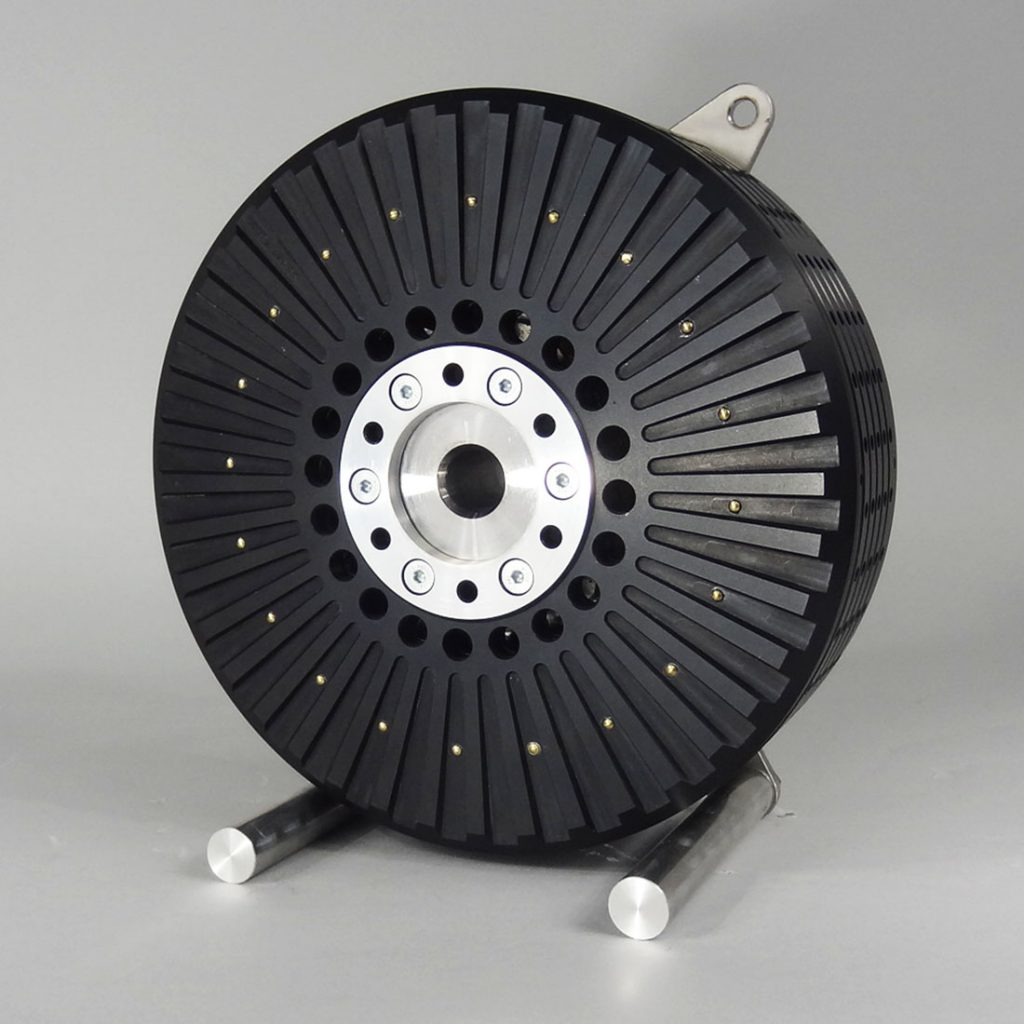
\includegraphics[width=0.5\textwidth]{images/fig4}
        \caption{Side profile of EMRAX 268 Axial Flux Electric Motor}
    \end{figure}
    \begin{figure}[H]
        \centering
        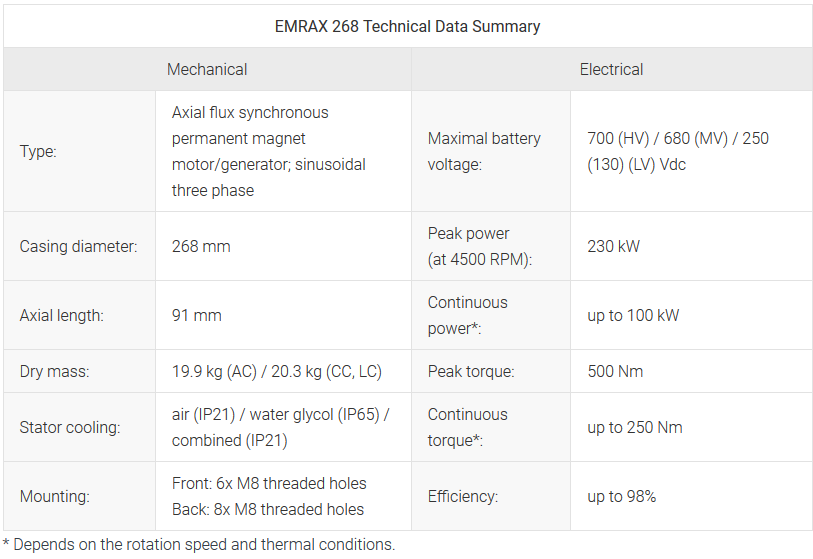
\includegraphics[width=\textwidth]{images/fig5}
        \caption{Summary of EMRAX 268 motor technical data [1]}
    \end{figure}
    \begin{figure}[H]
        \centering
        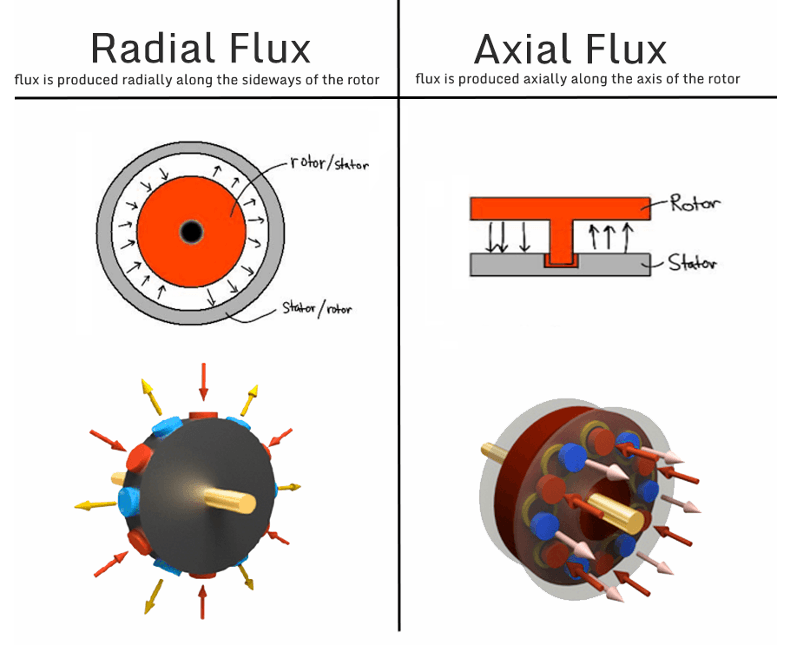
\includegraphics[width=\textwidth]{images/fig6}
        \caption{Axial Flux Motors are built similarly in the same fashion that regular permanent magnet motors are. However, the positions of the stator and rotors are reversed, where the outer casing is the rotor and the inner core is the stator. In addition, most electric motors are radial flux motors where the magnetic flux is oriented along the radial of the stator. Axial flux, as said in the name, orient their magnetic flux axially around the axis of the rotor [2]}
    \end{figure}
    \begin{figure}[H]
        \centering
        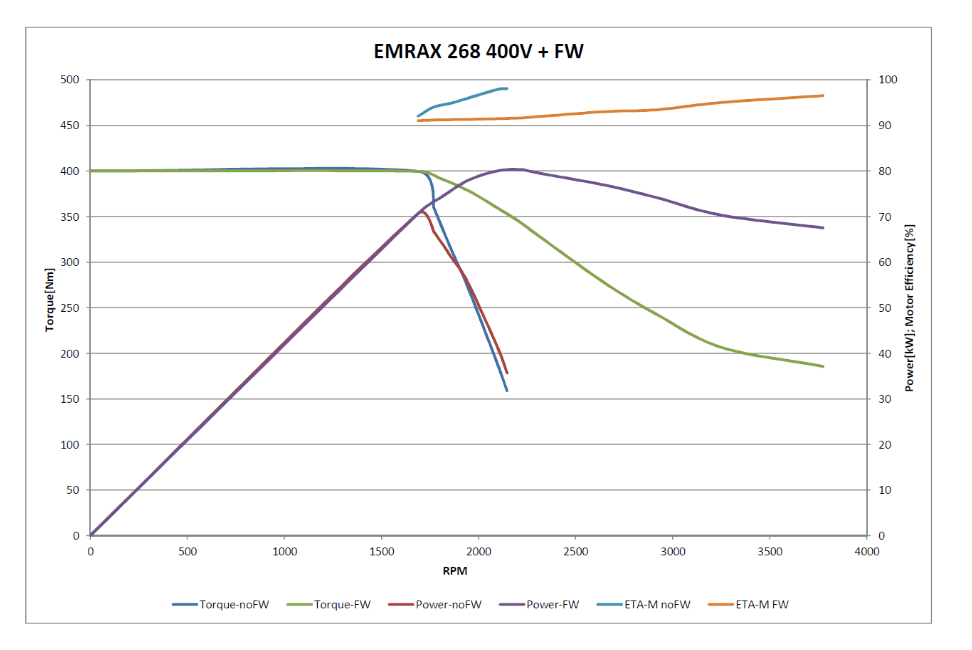
\includegraphics[width=\textwidth]{images/fig7}
        \caption{EMRAX 268 Torque/Mechanical Power/ Efficiency over RPM [3]}
    \end{figure}
    \subsubsection{Motor Performance}
    The graph above shows the torque, power and efficiency of the motor over RPM. As mentioned previously, the motor is capable of producing instantaneous torque, a peak of 400 Nm can be seen in the graph. EMRAX states that the motor is capable of greater RPM ranges by utilizing MFW (magnetic field weakening). The effect of MFW is significant in reducing the decay of torque at higher RPM ranges, and producing higher mechanical power. This is accomplished by reducing the overall efficiency of the motor. However, the reduction is not significant (<8\% greater loss), and the gains in performance outweigh the loss in efficiency.
    \begin{figure}[H]
        \centering
        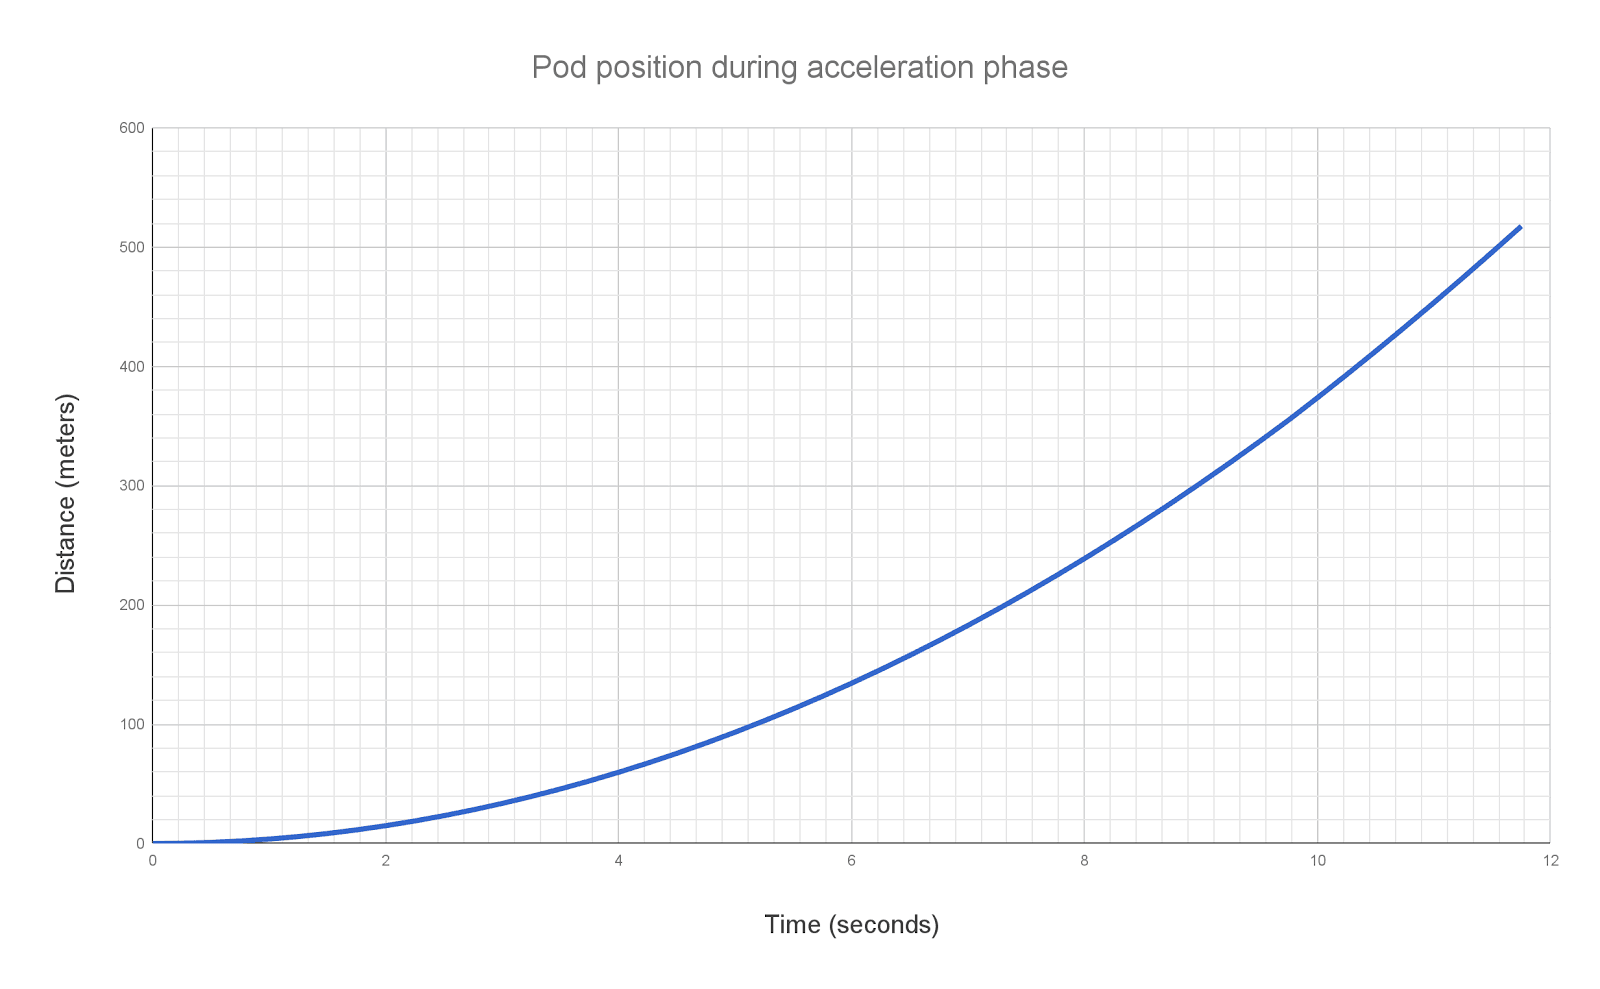
\includegraphics[width=\linewidth]{images/fig8}
        \caption{Pod position during acceleration phase}
    \end{figure}
    \begin{figure}[H]
        \centering
        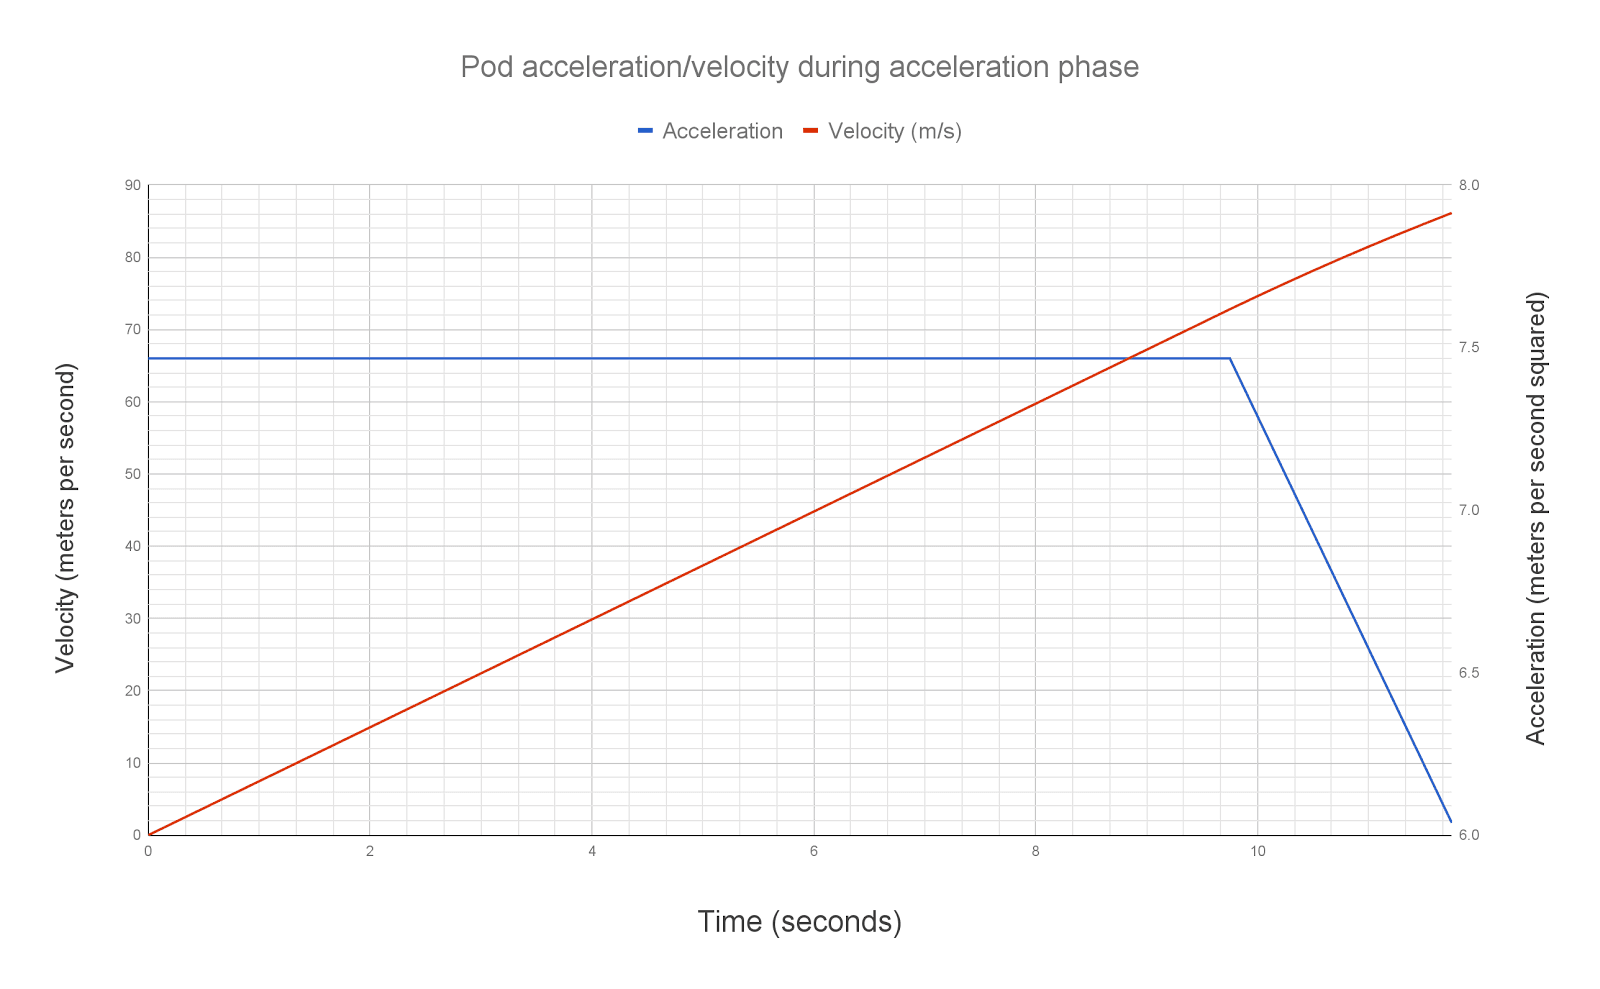
\includegraphics[width=\linewidth]{images/fig9}
        \caption{Pod acceleration/velocity during acceleration phase}
    \end{figure}
    \begin{figure}[H]
        \centering
        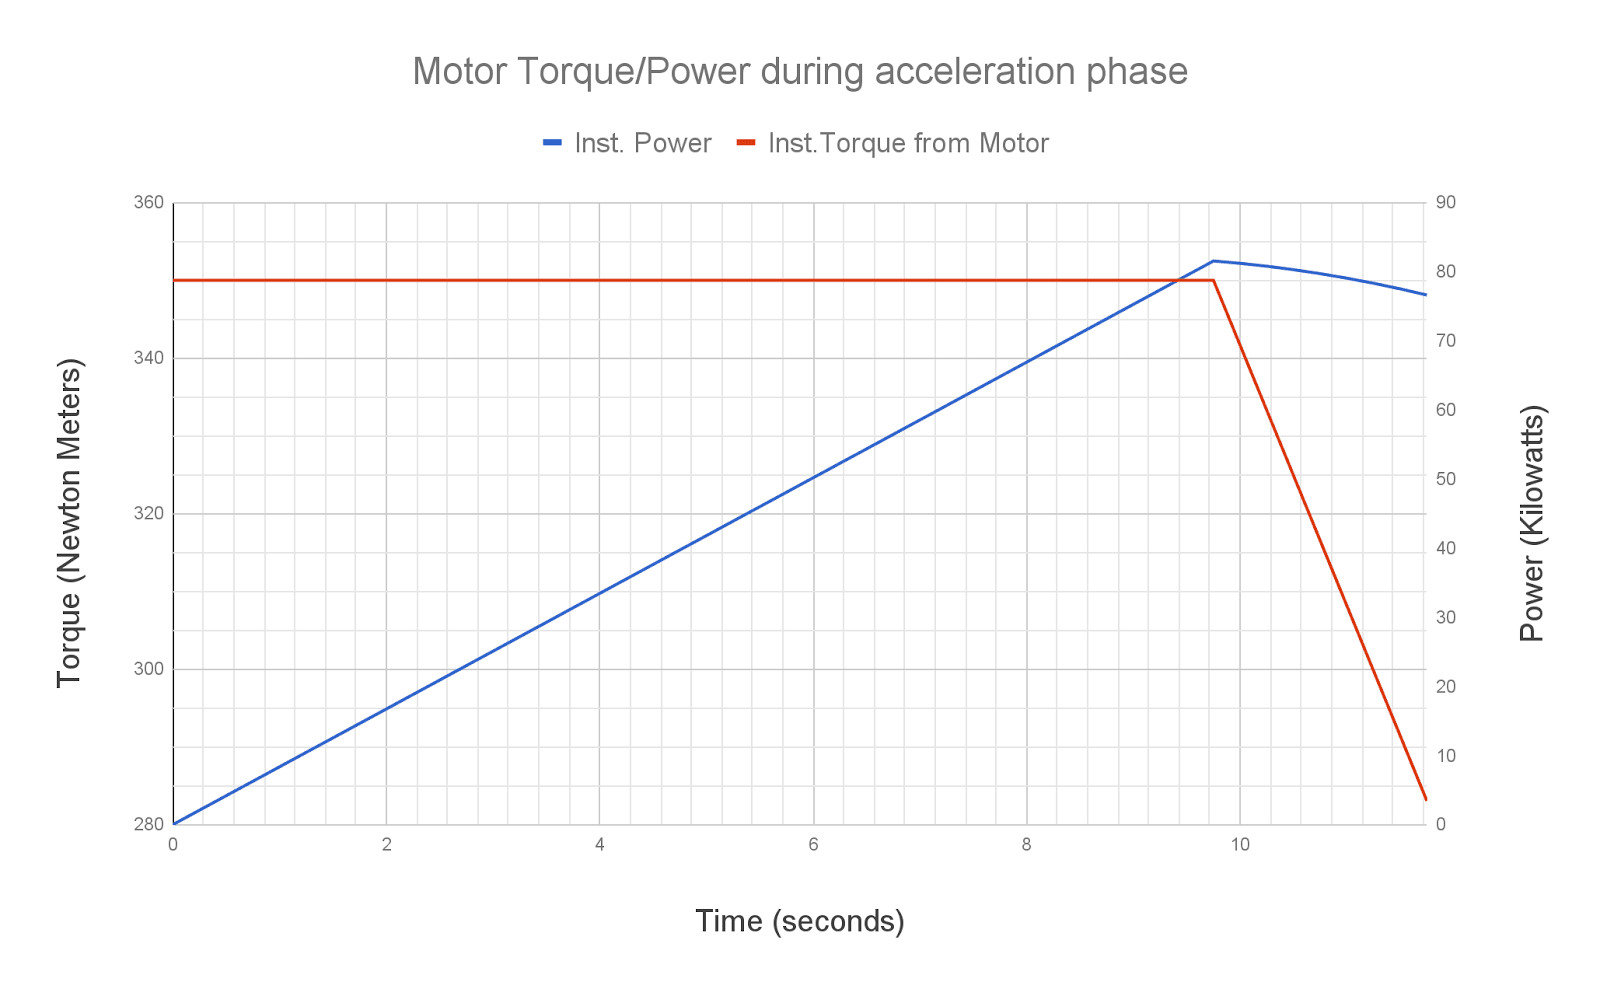
\includegraphics[width=\linewidth]{images/fig10}
        \caption{Motor Torque/Power during acceleration phase}
    \end{figure}
    \begin{figure}[H]
        \centering
        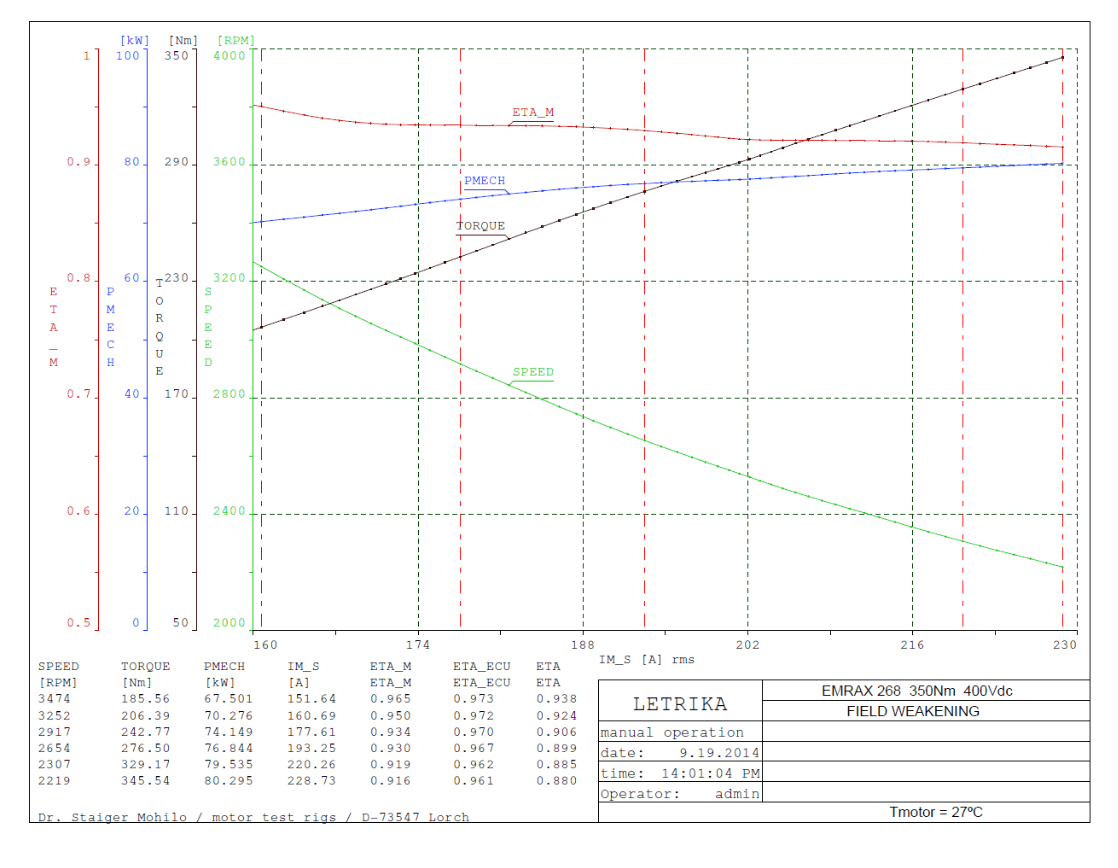
\includegraphics[width=\linewidth]{images/fig11}
        \caption{Caption needed}
    \end{figure}
    \subsection{Power Delivery}
    The EMRAX 268 has a variety of shaft mounting solutions. The most practiced ones are bolted flange shafts or a shaft within the splined hub of the motor. The flanged shaft was the choice for the design because of the ease at which one can assemble and perform maintenance on the powertrain and the versatility to alter shaft lengths and dimensions. In addition, in order to secure pulleys onto this shaft, the option of splining a shaft is available, which provides the most secure and efficient method of securing the pulleys. The shaft is made out of hardened steel (42CrMo4QT) which is commonly used to make driveshafts, turbocharger gears, crankshafts, etc.
    \begin{figure}[H]
        \centering
        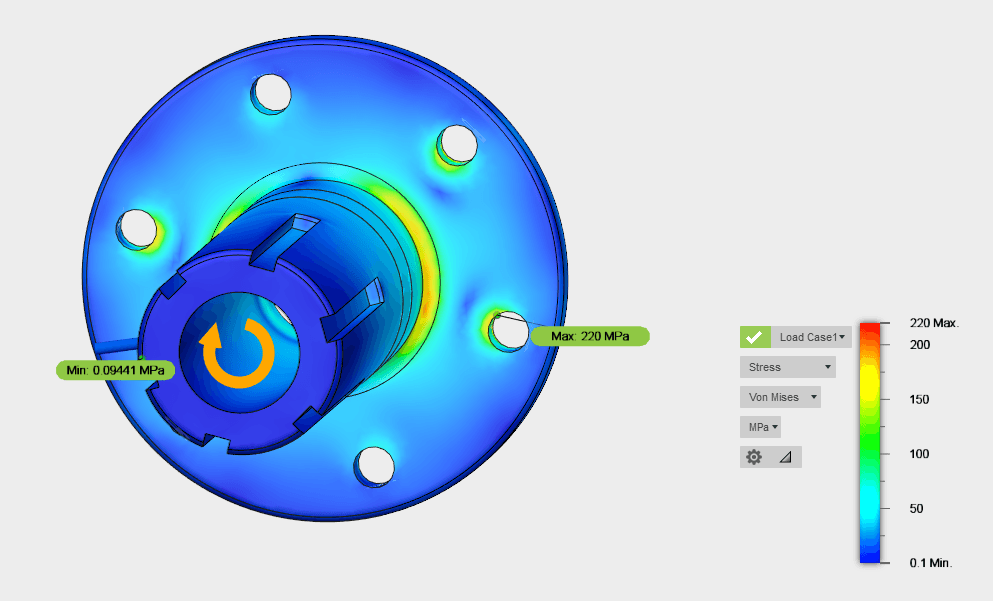
\includegraphics[width=\linewidth]{images/fig12}
        \caption{Caption needed}
    \end{figure}
    \subsubsection{Motor Shaft}
    Static stress FEA was done, in Autodesk Fusion 360, on the shaft in order to analyze stress concentrations and possible failures. The shaft was fixed via the bolt holes within the flange and the load was equivalent to the tension force that the pulley and belt system would exhibit at peak loads. In addition, an angular load was placed onto the shaft, equivalent to the maximum possible RPM range the motor could produce, which is about 1000 rad/s.\\
    
    The shaft experiences a peak stress of 220 MPa, located at the bolt holes on the flange. This raises concern regarding bolts that fasten the shaft to the motor. Reaction force was measured to be a peak of around 400N on the bolt, which means based on the cross sectional area of the bolt, shear force and moment, it would experience a peak of 338 MPa. This is within the yield strength of the bolt which is >965 MPa yield strength, exhibiting a safety factor around 3.
    \begin{figure}[H]
        \centering
        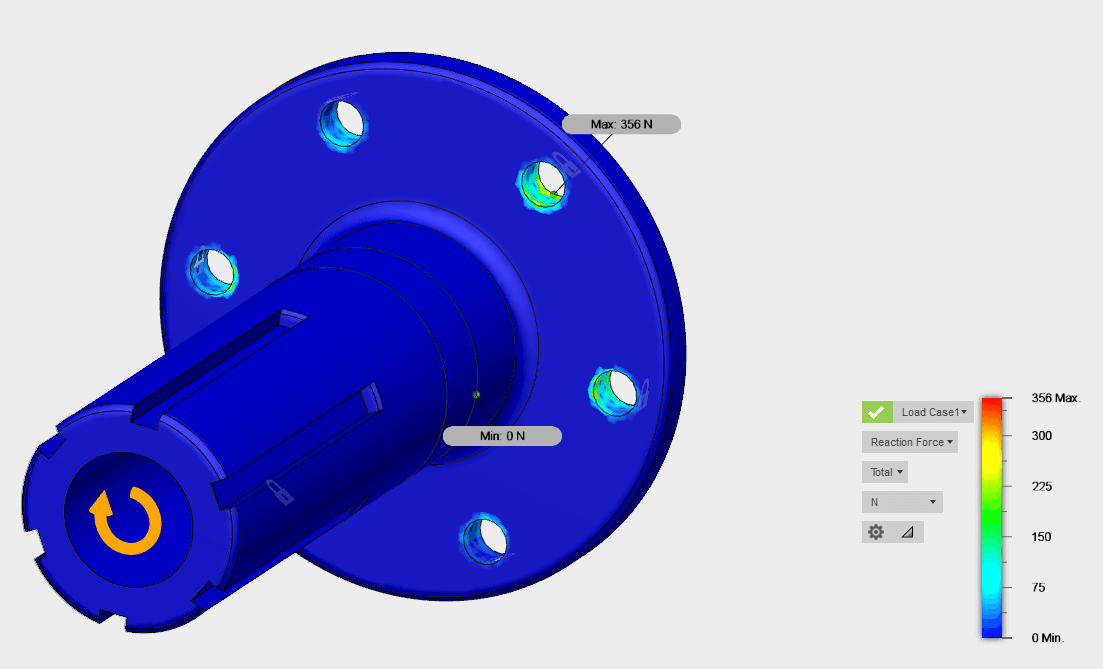
\includegraphics[width=\linewidth]{images/fig13}
        \caption{Caption needed}
    \end{figure}
    \begin{figure}[H]
        \centering
        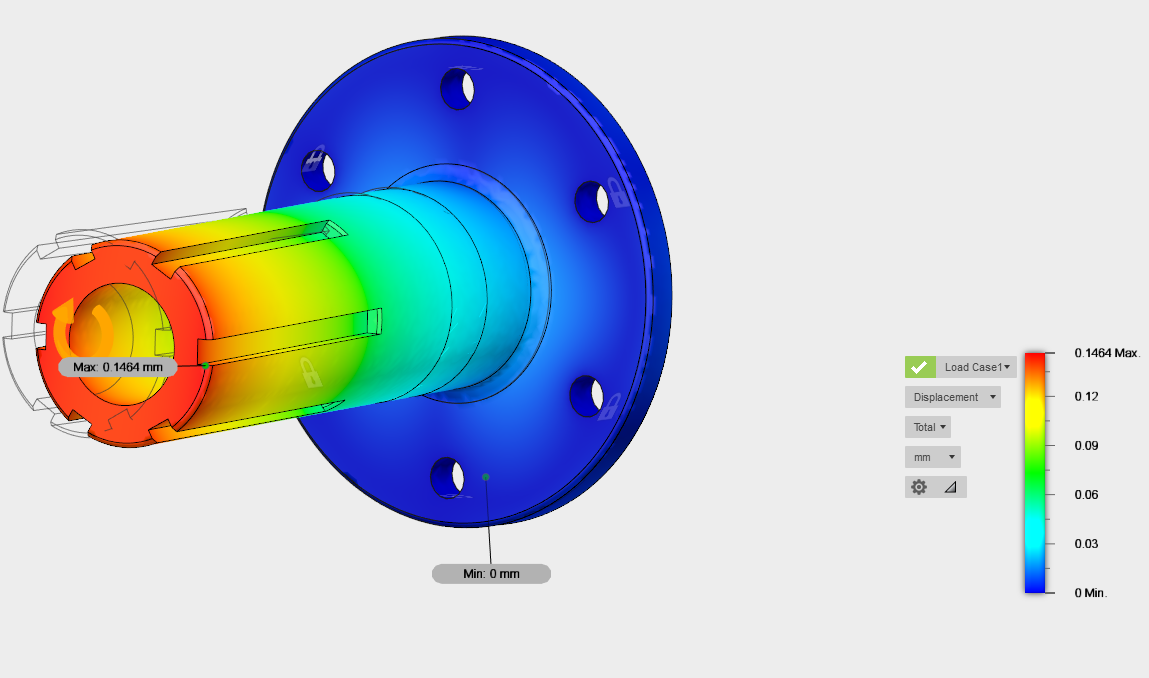
\includegraphics[width=\linewidth]{images/fig14}
        \caption{Caption needed}
    \end{figure}
    This is the displacement result of the FEA, where the peak displacement of the shaft is 0.15mm at the tip of the shaft. In the figure above, it is at a 5\% model based displacement adjustment. The mesh was created with an average element size of 3\% of the model based size had a parabolic element order. To refine our mesh and create more accurate results, adaptive mesh refinement was done in the areas of peak stress, at a cycle of 3 mesh refinements with a convergence tolerance of 5\%. Similar FEA was done on the other power transmission shaft that connects to the wheel. The result yielded less overall stress on the bolt holes due the shaft not having a hollowed core (200 MPa)
    \begin{figure}[H]
        \centering
        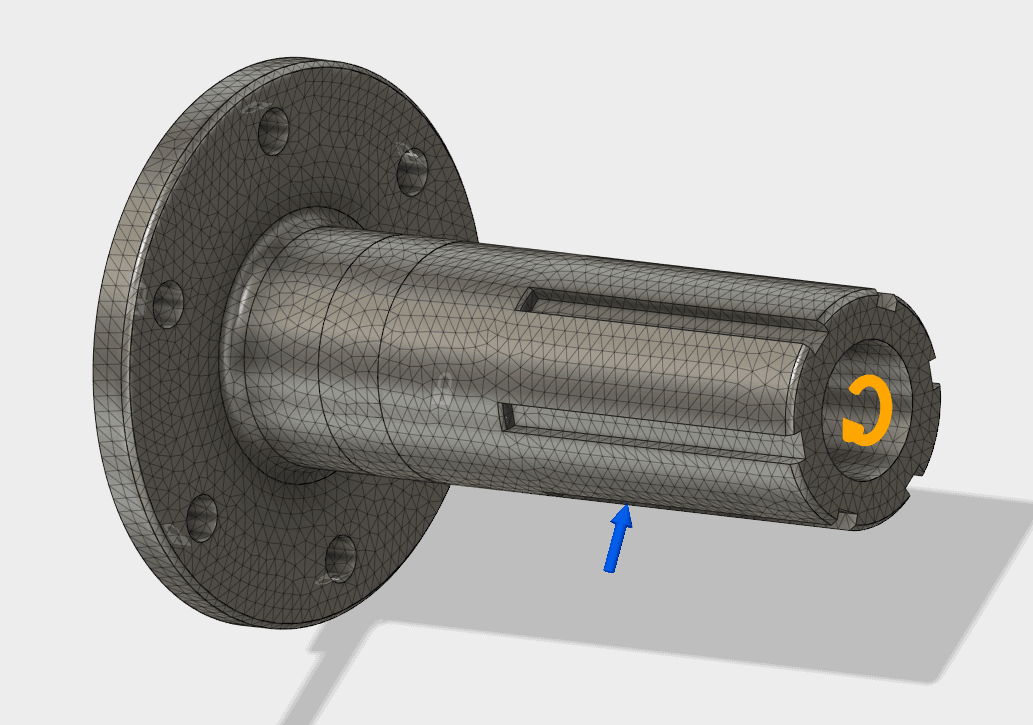
\includegraphics[width=\linewidth]{images/fig15}
        \caption{Caption needed}
    \end{figure}
    The mesh was created with an average element size of 3\% of the model based size had a parabolic element order. To refine our mesh and create more accurate results, adaptive mesh refinement was done in the areas of peak stress, at a cycle of 4 mesh refinements with a convergence tolerance of 5\%. 
    
    \subsubsection{Pulley}
    \begin{figure}[H]
        \centering
        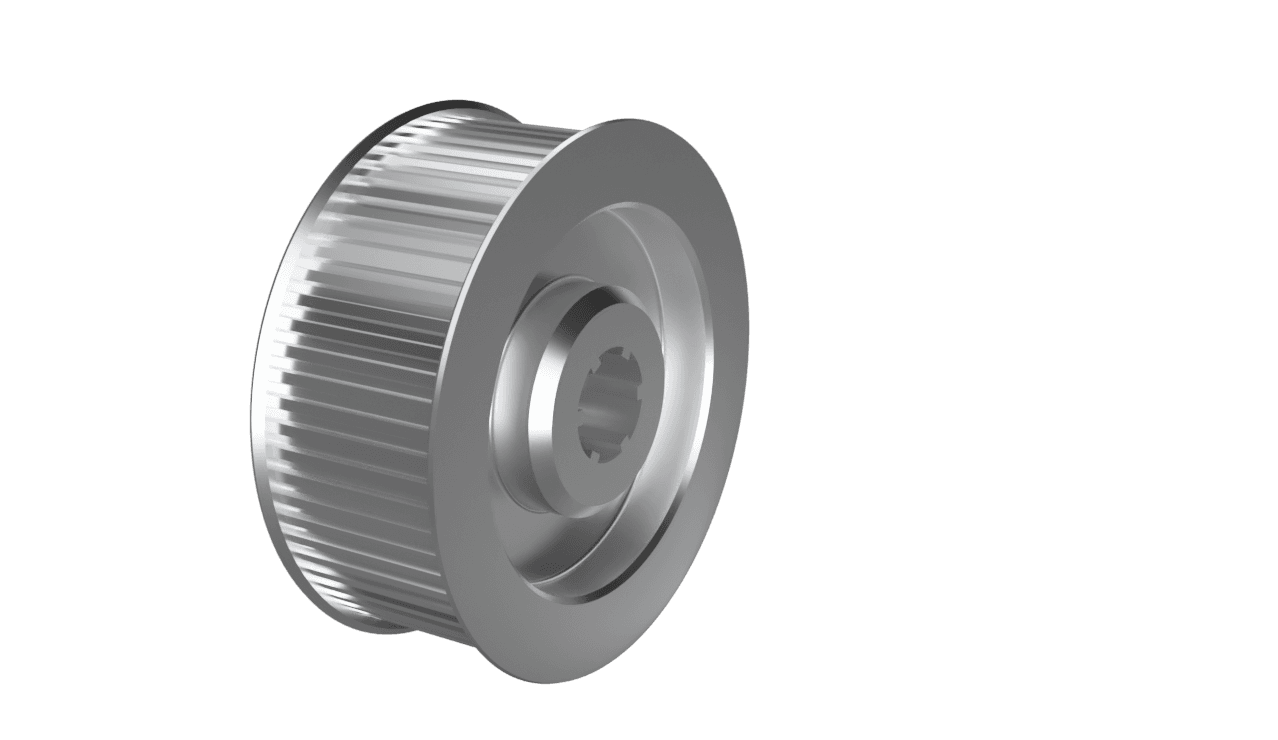
\includegraphics[width=\linewidth]{images/fig16}
        \caption{Caption needed}
    \end{figure}
    The propulsion system utilizes a single gear reduction in an open belt system, that incorporates an idler pulley to maintain contain tension on the system. Many different power transmission options were investigated, including a multi-gear system and a continuously variable transmission (CVT) system. However, these options were not chosen due to the overall complexity that these systems would have, and the costs and research \& development time involved in developing these systems would be far beyond the timeline allocated by the competition. Thus, a single gear reduction with the open belt system was chosen for the simplicity of design and testing, and the reduction of overall costs in integrated this power transmission system onto the pod.
    
    \paragraph{Vacuum Compatibility}
    We have identified two potential issues with the motor in vacuum, which we have discussed with the manufacturer EMRAX.
    \begin{itemize}
        \item Cooling of the motor may be designed for air environments, where air convection plays a role in addition to the liquid cooling system.
        \begin{itemize}
            \item EMRAX believes that due to the very short runtime (less than 30 seconds) there will be no significant difference in the efficacy of the cooling system in vacuum.
            \item They have also suggested that no cooling system is needed at all, and the heat capacity of the motor itself is enough to last 30 seconds without reaching 50 degrees Celsius. We decided to design a cooling system anyway, on the grounds that it would be prudent to have and could be relatively trivially removed if physical tests showed it to be significantly redundant.
        \end{itemize}
        \item Outgassing of the epoxy used to secure the motor’s internal components could weaken these fastenings and also deposit epoxy on other parts of the motor.
        \begin{itemize}
            \item EMRAX has confirmed that the motor’s internal components are both mechanically and chemically secured, so that even with epoxy outgassing there will be no problems in fastening.
            \item Deposition of epoxy could damage other parts within the motor. [CAN WE ASK THEM WHAT THINGS THEY ARE USING THAT COULD OUTGAS?]
        \end{itemize}
    \end{itemize}
    
    \subsection{ESC}
    EMRAX recommended several electronic speed controllers (ESC) and the UniTek Bamocar D3 stood out due to its low-cost and well-balanced performance. The controller weighs 6.8 kilograms and accepts a voltage input of up to 700 V, with a continuous current of 200 A. The controller also comes with a liquid cooling system that is situated at the bottom of the controller.
    \begin{figure}[H]
        \centering
        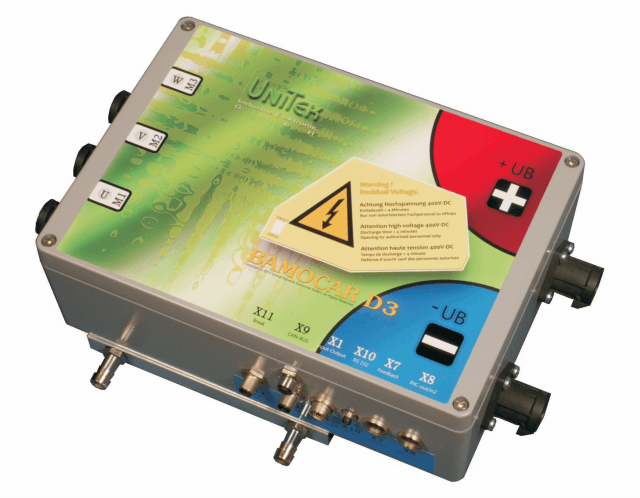
\includegraphics[width=\linewidth]{images/fig17}
        \caption{Caption needed}
    \end{figure}
    
    \subsection{Cooling System}
    Cooling system; heat transfer calcs results; thermal simulation would be nice [including ESC and motor]\\
    
    The cooling system is designed to be as safe as possible by offering ample cooling while also making it easy to assemble and maintain. The EMRAX 268 specifies limits to the flow rate and pressure of the cooling loop with a flow rate of 8 litres per minute at 2 bars accounting for vacuum, the loop will be running at 7 litres per minute at 1.5 bars to stay under these limits. The cooling loop(figure ?) is a series loop with no parallel lanes, allowing for a simple to install and clean path for a 25/75 glycol/water solution as coolant. The loop will be using multiple temperature and pressure sensors to ensure the coolant will never exceed the pressure or temperature limit of the motor of 2 Bar and motor inlet coolant temperature of \SI{50}{\celsius}. If the 2 bar pressure limit is reached, a solenoid valve will be opened to release some coolant into a release tank, allowing pressure inside the cooling loop to be lowered. In the event of the temperature limit being reached, the motor and controller settings will be lowered to allow for heat to be dissipated from the loop and the temperature to be lowered. A ball valve is also present in order to completely stop the flow of coolant when the power is off and the pod is not running.
    \begin{figure}[H]
        \centering
        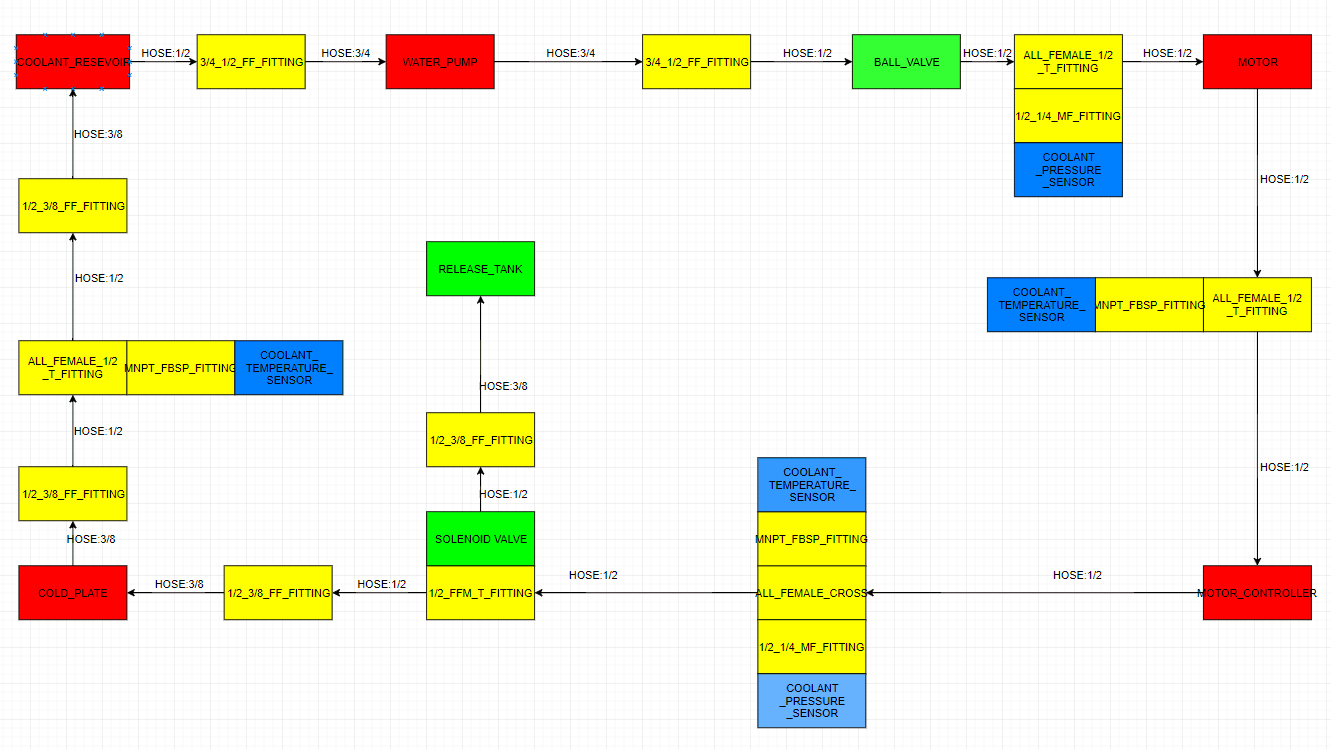
\includegraphics[width=\linewidth]{images/fig18}
        \caption{The cooling loop uses fittings and hoses in order to move from one component to the next seamlessly}
    \end{figure}
    The design parameters of the cooling system used worst-case-scenario heat dissipation numbers: the motor uses 100 kW at peak, with specified minimum 92\% efficiency, with the motor controller introducing a maximum of 3 kW,  so we must dissipate 11 kW during a maximum run time of 20 seconds. Using these values and assuming no heat is dissipated through the cold plate and tubing, the total heat input to the loop was calculated using
    \[
    Q = mc \Delta T
    \]
    where $Q$ is \SI{220}{kJ}, $c$ is \SI{3.85}{kJ/kgK} for a 25/75 water/glycol solution at \SI{25}{\celsius}, $m$ is mass of coolant required, and $\Delta T$ is \SI{25}{\celsius}. The mass of coolant required is approximately \SI{2.3}{kg} or $\sim$\SI{2.3}{L}. A 2 litre reservoir was chosen to make up most of the required coolant with the volume of the tubing adding the rest and more. In addition, a cold plate is present in the loop as another safety and redundancy factor in the loop. With the tubing and cold plate dissipating heat, an extra 5 seconds of expected run time, and supplementary coolant mass, it can be estimated that the cooling loop will not exceed a delta temperature of \SI{25}{\celsius}, allowing for a safe acceleration and run of the pod.\\
    
    The cold plate will be attached to a beam on the ladder frame of the pod, acting as a metal block to absorb any heat that is created. With temperatures not exceeding \SI{50}{\celsius} in the loop before the addition of the coldplate, the aluminum beam will not experience any extreme heat, keeping the integrity of the frame and pod.
    
    \subsection{Wheel \& Slip}
    Wheel material, cost, fabrication (how are we doing polyurethane?)
    \begin{figure}[H]
        \centering
        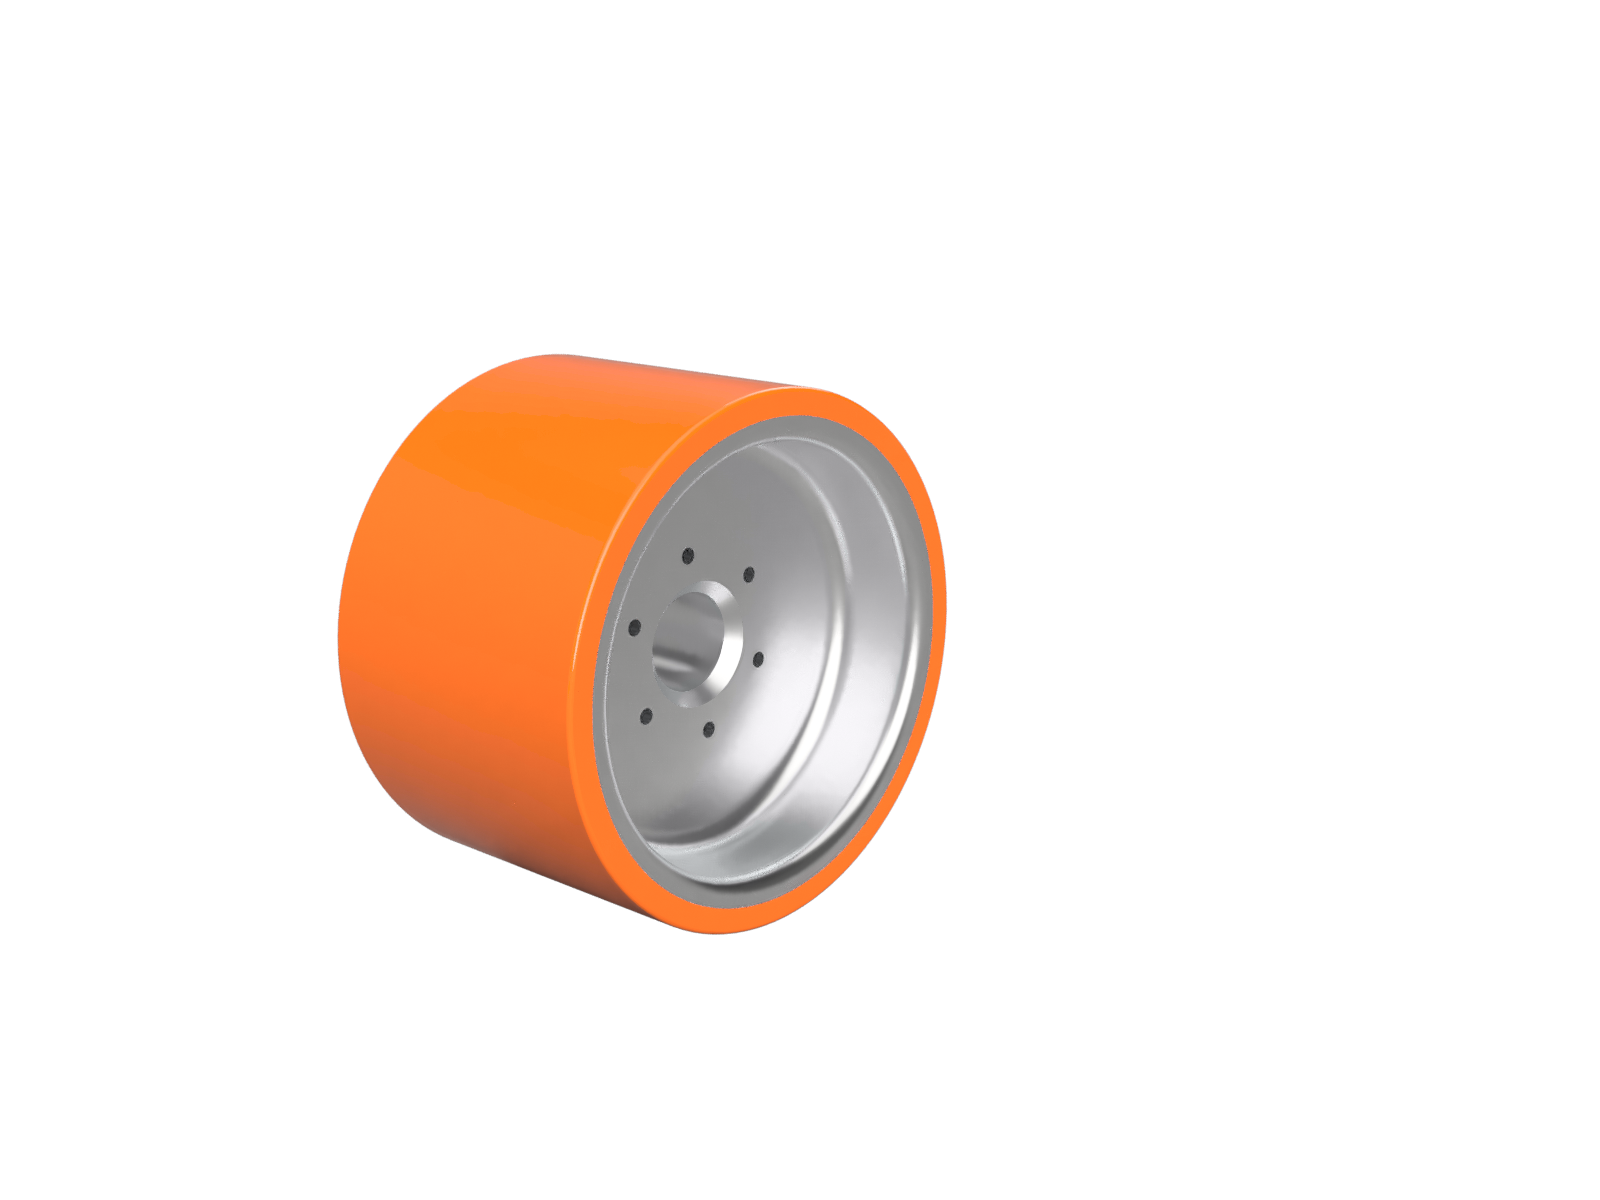
\includegraphics[width=\linewidth]{images/fig19}
        \caption{Caption needed}
    \end{figure}
    Our propulsion system requires strong wheels that are able to withstand high RPM ranges at a large variety of axial and thrust loads. The design was created with an aluminum 6061-T6511 core and a polyurethane wheel tread. Aluminium 6061-T6511 was chosen as the wheel’s core because of the yield strength and low density as we would require the wheel to be lightweight in order to minimize inefficiency of transferring torque to the ground and the strength such that the wheel will not yield under peak loads. In addition, because this material is easily machined, there is no need for extensive tooling or custom extrusion techniques in order to produce the wheel. 6061-T6511 is a well known and common alloy and thus extensive research has been conducted on the fatigue behaviour of this wheel. Based on fatigue analysis\footnote{ https://www.osti.gov/scitech/servlets/purl/10157028}, even when the wheel has done $10^6$ cycles, it will still be within design specifications and can be used safely.\\
    
    Testing for the wheel (balance issues?)
    
    \paragraph{Calculations for slip}
    By using first-principles of newtonian physics, we can simplify our traction based on static friction. In order to translate angular movement into translational movement, we require that the wheel remain in traction with the track.\\
    
    Where the overall mass, $m$, of the pod is \SI{150}{kg} and 65\% of the weight is biased towards the drive wheel.
    
    \begin{center}
        We want to achieve an acceleration of \SI{1}{g} or \SI{9.8}{m/s^2}\\
        
        Thus, $F_a=m\cdot a = \SI{150}{kg} \times \SI{9.8}{m/s^2} = \SI{1500}{N}$\\
        
        Frictional force is calculated via $F_f=\mu_s \times F_n$. In this case, $F_f=F_a=\SI{1500}{N}$\\
        
        Based on the static coefficient of friction of 0.7 with polyurethane vs aluminum,
        \[
        F_n = \frac{F_f}{\mu_s} = \frac{\SI{1500}{N}}{0.7} \approx \SI{2200}{N}
        \]
        
        But with 65\% biased on the drive wheel, only $\SI{1500}{N} \times 0.6 = \SI{975}{N}$\\
        
        But we have a deficit in normal force. $\SI{2200}{N} -\SI{975}{N}=\SI{1225}{N}$
    \end{center}
    Based on these calculations, we required that we increase the normal force between the wheel and the rail in order to achieve our nominal acceleration of around 1 g and to prevent slipping of the drive wheel.\\
    
    The wheel core will be machined from an aluminum billet on a CNC. This will be fairly simple to achieve, and does not require any special tooling or machining processes to accomplish. In addition, this allows the balancing of the wheel to be easily achievable due to the lack of manufacturing errors that are produced by casting the wheel. In order to produce the polyurethane tread, we must create a mold and cast the polyurethane tread. This tread will then be chemically secured to the aluminum wheel via vacuum grade epoxy. This process takes the majority of the cost associated with producing the wheel- however, the possibility of machining the tread out of a solid block of polyurethane is currently being investigated as it as a vastly more cost effective solution.
    
    A solution to our normal force deficit: Pneumatic Actuators
    \begin{figure}[H]
        \centering
        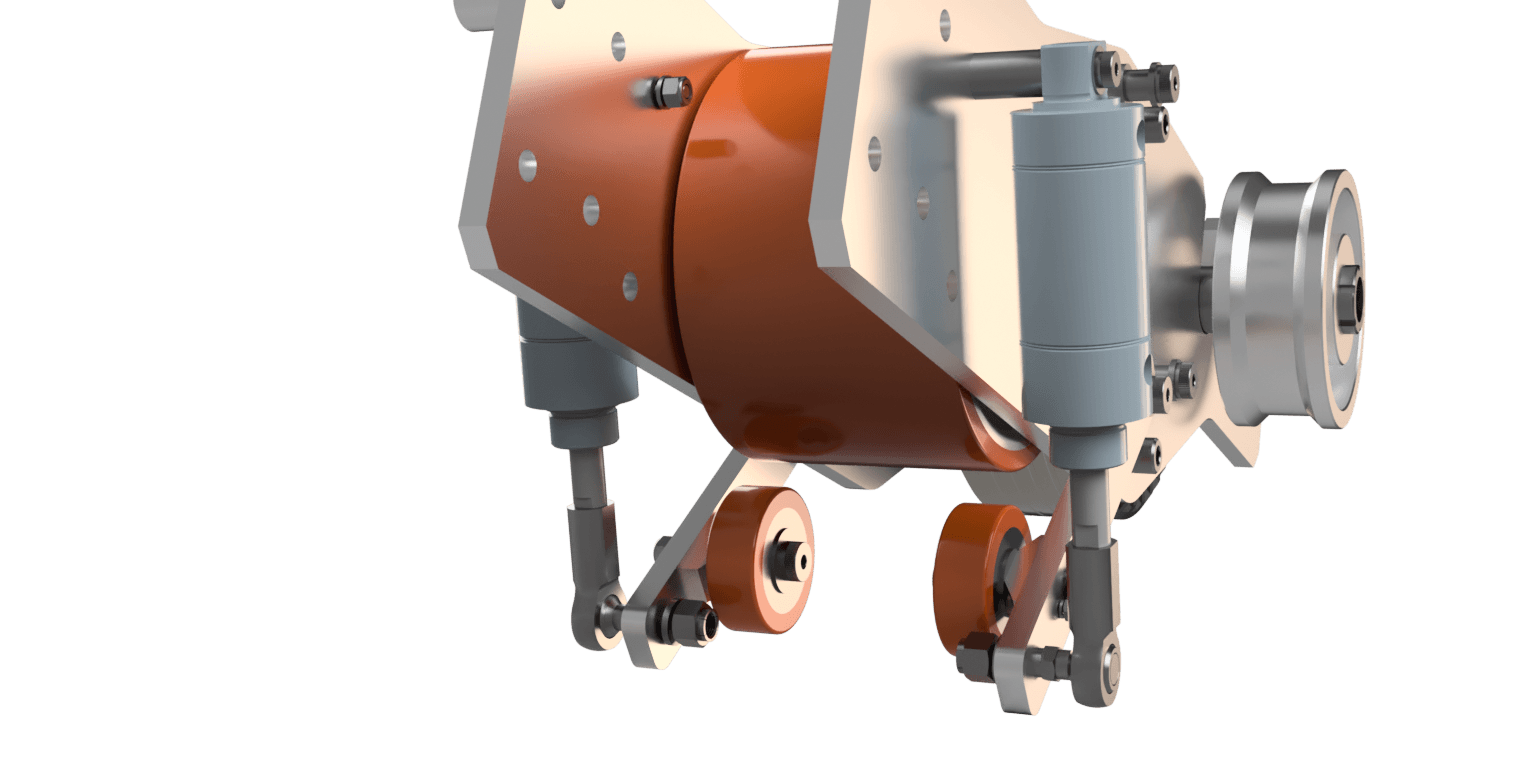
\includegraphics[width=\linewidth]{images/fig20}
        \caption{Caption needed}
    \end{figure}
    By utilising a guide wheel under the I-beam and a pneumatic actuator fastened to a pivot arm to clamp down onto the I-beam flange, we are able to increase the theoretical normal force that the wheel can provide and thus increase our static frictional force. The pneumatic actuator allows us to modulate the traction force needed and dampen any impacts that the guide wheels will encounter moving down the track.
    
    \paragraph{Pneumatic Circuit}
    Is there a way to do both centripetal and shear FEA on the polyurethane?\\
    \begin{figure}[H]
        \centering
        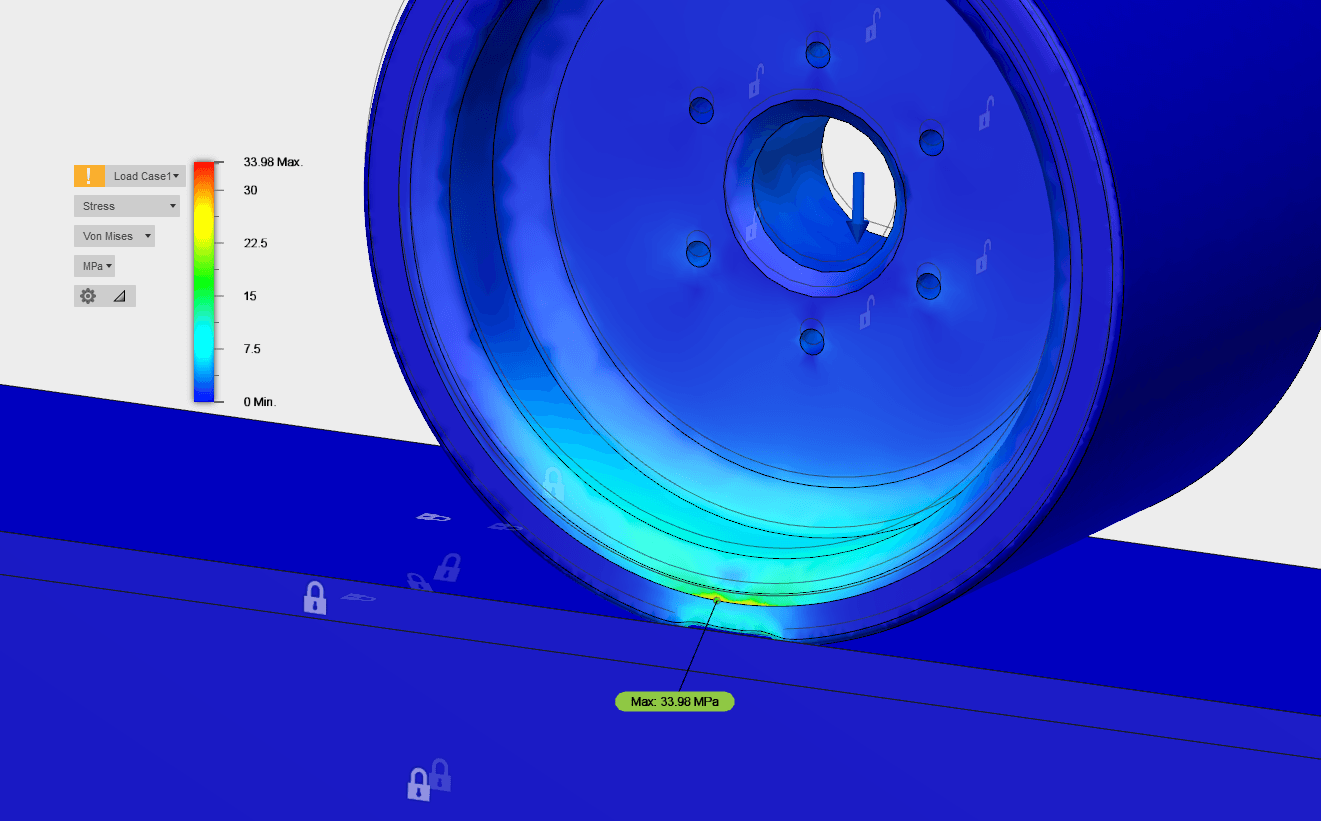
\includegraphics[width=\linewidth]{images/fig21}
        \caption{Static Stress FEA, Peak compressive load on main drive wheel}
    \end{figure}
    This finite element analysis was conducted, in Autodesk Fusion 360, by placing a compressive load onto the wheel equivalent to the weight of the pod, plus the force that the pneumatic actuators would provide in order to create the required traction force. The track was grounded and fixed in all orthogonal directions and the wheel fixed via the bolt fixtures within the aluminum core.\\
    
    The aluminum core only experiences a peak stress of \SI{34}{MPa}, which is significantly lower than the yield strength of the material, \SI{275}{MPa}, and provides a safety factor of over 8. The polyurethane tread is a hardness of \SI{90}{A} on the Shore hardness scale. The tread experiences a peak stress of \SI{17}{MPa}, where as the tensile strength of the tread material is \SI{50}{MPa}, giving us a suitable safety factor of around 3.
    \begin{figure}[H]
        \centering
        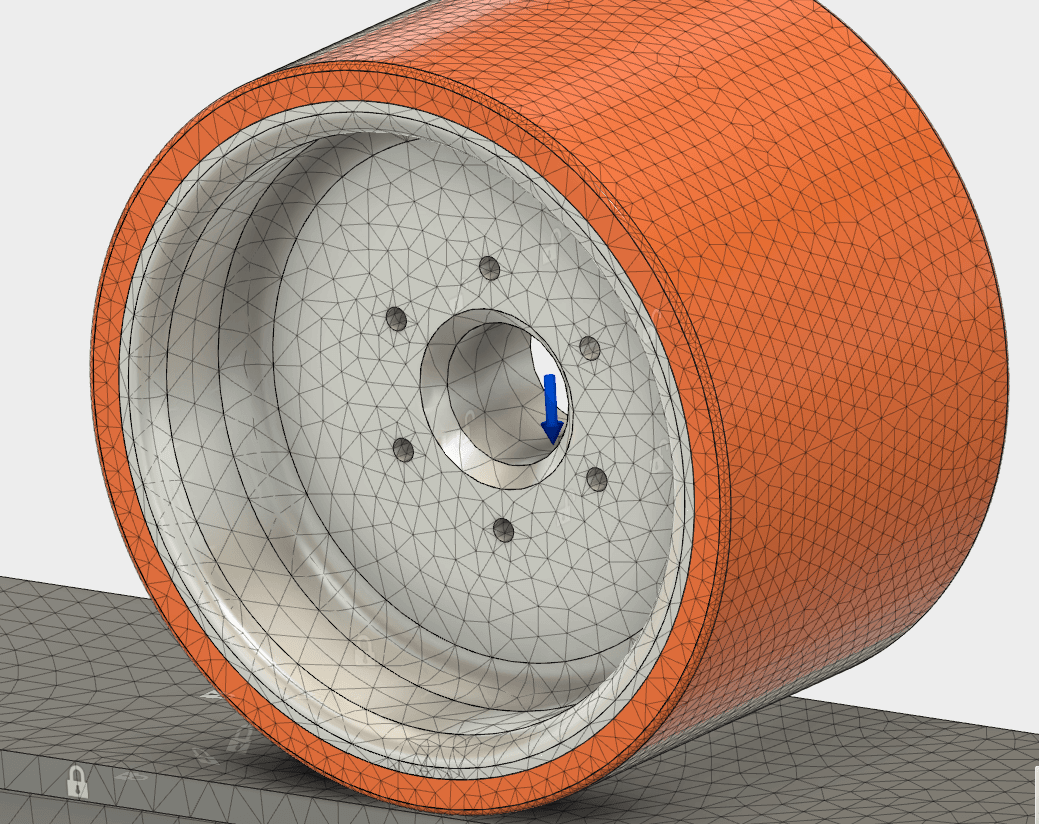
\includegraphics[width=\linewidth]{images/fig22}
        \caption{Caption needed}
    \end{figure}
    The mesh was created with an average element size of 2\% of the model based size had a parabolic element order. To refine our mesh and create more accurate results, adaptive mesh refinement was done in the areas of peak stress, at a cycle of 6 mesh refinements with a convergence tolerance of 5\%.

    \paragraph{Wheel balancing}
    \subsection{Friction Braking Calipers}
    \begin{figure}[H]
        \centering
        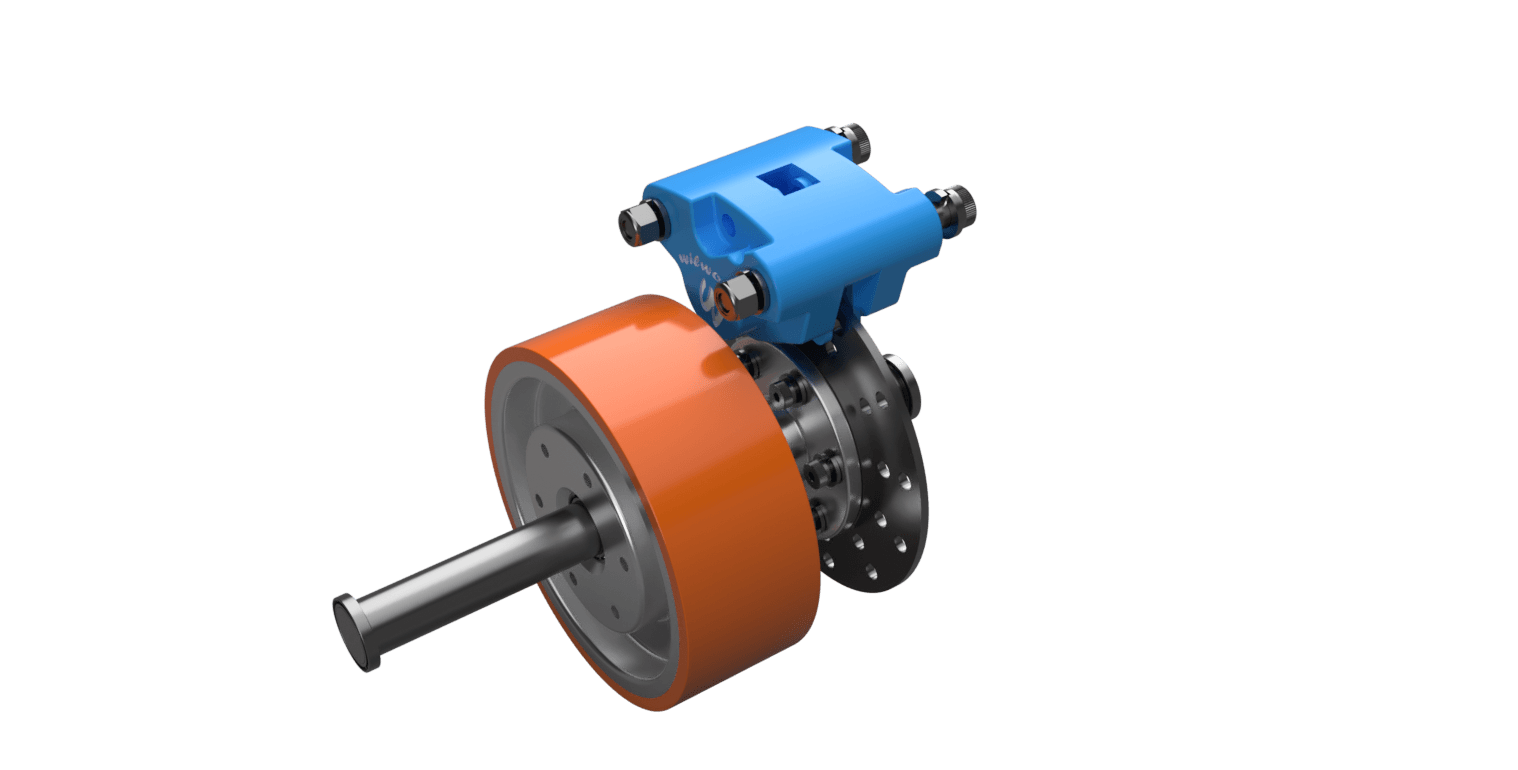
\includegraphics[width=\linewidth]{images/fig23}
        \caption{Caption needed}
    \end{figure}

    \paragraph{Motivation}
    Due to Eddy Current Brakes (see below) being ineffective at speeds below 5 m/s, the pod required a secondary braking source to bring it to a complete stop. Friction brake calipers were determined to be the most simple and effective solution, with many off-the-shelf components available. The brakes are not required to perform at high speeds, and as such, do not require large brake rotors or high performance calipers/pads in order to stop the vehicle  As such, there is no requirement to create a custom braking system and the cost associated with creating such a braking system are minimal. It is easily integrated into the original design, requiring little to no alteration to major drivetrain components.\\
    
    \paragraph{Heating}
    The kinetic energy before friction brake is activated is given by: $\frac{1}{2}mv^2=12(150)(10)^2=\SI{1875}{J}$\\
    When the friction brake is activated, kinetic energy will be converted to heat, which will be transferred to the brake rotor disc and the brake pad.
    Although the manufacturer did not specifically state the material composition, gray cast iron is the most common material for brake rotor discs. A rough estimation of the composition of such material, and the density and specific heat capacity of each metallic element, are as follows:\\
    
    \begin{table}[H]
        \centering
        \begin{tabular}{@{}lrrrrrr@{}} \toprule
            Element & Iron & Carbon & Silicon & Manganese & Phosphorus & Sulfur\\ \midrule
            \% Weight & 93.487\% & 3.4\% & 2\% & 0.58\% & 0.51\% & 0.023\%\\
            Density (\si{g/mm^3}) & 0.007874 & 0.00226 & 0.00233 & 0.00747 & 0.00196 & 0.001823\\
            Specific Heat Capacity (\si{J/(g\celsius)}) & 0.449 & 0.71 & 0.71 & 0.479 & 0.705 & 0.770\\ \bottomrule
        \end{tabular}
        \caption{Caption needed}
    \end{table}
    
    Using the dimensions provided by the manufacturer, the volume of the brake rotor disc can be found.
    \[
    4\pi(63)^2-\pi(23.5)^2-120\pi(3.175)^2=\SI{44340}{mm^3}
    \]
    The mass and specific heat capacity of the brake rotor disc can be found using the percentage weight, density and specific heat capacity of each element.
    \begin{gather*}
    \mathrm{Mass} = \frac{44340}{\frac{0.034}{0.00226} + \frac{0.02}{0.00233} + \frac{0.0058}{0.00747} + \frac{0.0051}{0.00196} + \frac{0.00023}{0.001823} + \frac{0.93487}{0.007874}} = \SI{303.6}{g}\\
    \textit{SHC}=0.71(0.034)+0.71(0.02)+0.479(0.0058)+0.705(0.0051)+0.770(0.00023)+0.449(0.93487)=0.465
    \end{gather*}
    Although the brake pad uses sintered metallic material, the material composition is kept confidential by the manufacturer. The composition is drastically different between manufacturers, thus it is rather hard to make an appropriate estimation. Some of the common primary materials are graphite, copper and iron. Carbon steel serves as a decent balance among the three materials, and thus is used to make an approximation.\\
    
    The density of carbon steel is \SI{0.00785}{g/mm^3}, with a specific heat capacity of \SI{0.49}{J/(g\celsius)}. The volume of the brake pad is \SI{5572}{mm3}, which approximates the mass to be \SI{43.7}{g}.
    
    Using the heat transfer equation of $\Delta Q = mc \Delta T$,
    \[
    T=\frac{1875}{303.6(0.465)+43.7(0.49)}=\SI{11.5}{\celsius}
    \]
    The brake rotor disc and the brake pad will gain approximately \SI{1875}{J} of energy, and the temperature will increase by \SI{11.5}{\celsius}.\\
    
    https://willmanind.com/what-is-grey-cast-iron/\\
    http://periodictable.com/Properties/A/Density.al.html\\
    http://periodictable.com/Properties/A/SpecificHeat.html
    
    \paragraph{Failsafes}
    The solenoid that controls the brake master cylinder will be on an electrically failsafe circuit, in the case of power loss, there will be a reserved battery source to make sure that the calipers are actuated at the correct speeds. In addition, these brakes are mechanically failsafe. In the case of complete electrical power loss, the solenoid holding the calipers opens will be a normally open valve and will automatically actuate.
    
    \subsection{Tests \& Validation (completed and planned)}
    Test rig (see Next Steps as well)\\
    Fault tolerance, potential failure modes (FMEA)\\
    How will we verify that the OTS motor is in fact working to spec?\\
    How will we test all aspects of the motor?
    
    \section{Eddy Current Brakes}
    With only 1.6 kilometers of tube to work with, it’s extremely difficult to dissipate the huge kinetic energy at 100m/s so quickly. Pure friction braking, as with the braking calipers above, cannot work alone, since either the enormous shear forces and heat generated will destroy the brakes, or the pod will not stop within the length of the tube. [NUMBERS?] Eddy current brakes have the advantage of dissipating most of the kinetic energy of the pod into an external heatsink - the I-beams.
    
    \subsection{Overall Design}
    [Comments on how this integrates with friction braking calipers]\\
    Full labeled detailed CAD\\
    Mass, power, etc.\\
    How is it failsafe?\\
    Full cost breakdown, comments on manufacturability and production costs\\
    “A full Bill of Materials can be found in Appendix C.”
    
    \subsection{Physical Modeling}
    Fun magnet graphs!!\\
    Comparison of Force Velocity Graphs and A-t V-t D-t\\
    Thermal - I beam heat generation, show it will not be harmful
    
    \subsection{Structural}
    How is it failsafe?\\
    What are several reasonable and edge-case loading scenarios, and how does the FEA look for all of those? Justify your “reasonable” scenarios. If possible to simulate, how many cycles might it withstand?\\
    How will we deal with imperfections and irregularities in the track, both lateral and vertical? (Simulation would be good)
    
    \subsection{Tests \& Validation (completed and planned)}
    Test rig (see Next Steps as well)\\
    Fault tolerance, potential failure modes (FMEA)
    
    \subsection{Safety and handling}
    Magnet safety and handling procedures
    How do we verify that the magnets are magnetized enough? How do we preserve the magnetism?
    
    \section{Lateral}
    Why wheels?
    
    \subsection{Overall Design}
    Full labeled detailed CAD\\
    Mass, dimensions, etc.\\
    Full cost breakdown, comments on manufacturability and production costs\\
    “A full Bill of Materials can be found in Appendix C.”
    
    \subsection{Structural}
    “Fully passive, so failsafe in case of power or other failures.”\\
    How does the system effectively dampen lateral vibration? Simulations.\\
    \begin{itemize}
        \item Lateral response graph
    \end{itemize}
    High rpm issues, both structural and thermal\\
    What are several reasonable and edge-case loading scenarios, and how does the FEA look for all of those? Justify your “reasonable” scenarios. If possible to simulate, how many cycles might it withstand?
    
    \subsection{Tests \& Validation (completed and planned)}
    Test rig (see Next Steps as well)\\
    Fault tolerance, potential failure modes (FMEA)
    
    \section{Frame}
    The ladder frame is what we decided to go with, similar to our Competition 2 design. It consists of two L-Beams facing towards each-other with four I-Beam cross beams connecting them. There are a few major design changes that were made to adapt to changes in the pod subsystems. A longer frame was vital in the new design to accommodate the new friction drive propulsion system and the longer Eddy-Current Brakes. To avoid excessive torsional forces, and to simplify mounting of the friction drive and the shell, the frame was made narrower. For battery mounting, an additional flat plate crossmember was added parallel to the I-Beams. This flat plate was also vital for reducing deformities from the transverse forces of the EC Brakes.\\
    
    There was an investigation into using a honeycomb plate with sections cut out as the frame. While it would have been a very light alternative to the current ladder design, there were two major things holding us back from the decision. The first problem we ran into was the cost. The whole plate to be ordered would have been around \$4000, twice the anticipated expense for the frame. The other problem would be the complicated FEA associated with a honeycomb plate structure.  As a non isotropic material, the FEA would have taken a while to figure out and run. It was in our best interest to use our time to optimize the design of our ladder frame.\\
    
    The material used will be 7075 T6 for the I-beam crossmembers and 6061 T6 for the L-Beams. There was thought put into making the whole pod out of 6061 T6, similar to the competition 2 design, but due to the extreme forces from the EC-Brakes, the material had to be changed to 7075 T6 on the I-Beams. The 6061 T6 on the L-beams will be reasonable for our design, without increasing the cost of the frame too much.
    
    \subsection{Overall Design}
    \begin{figure}[H]
        \centering
        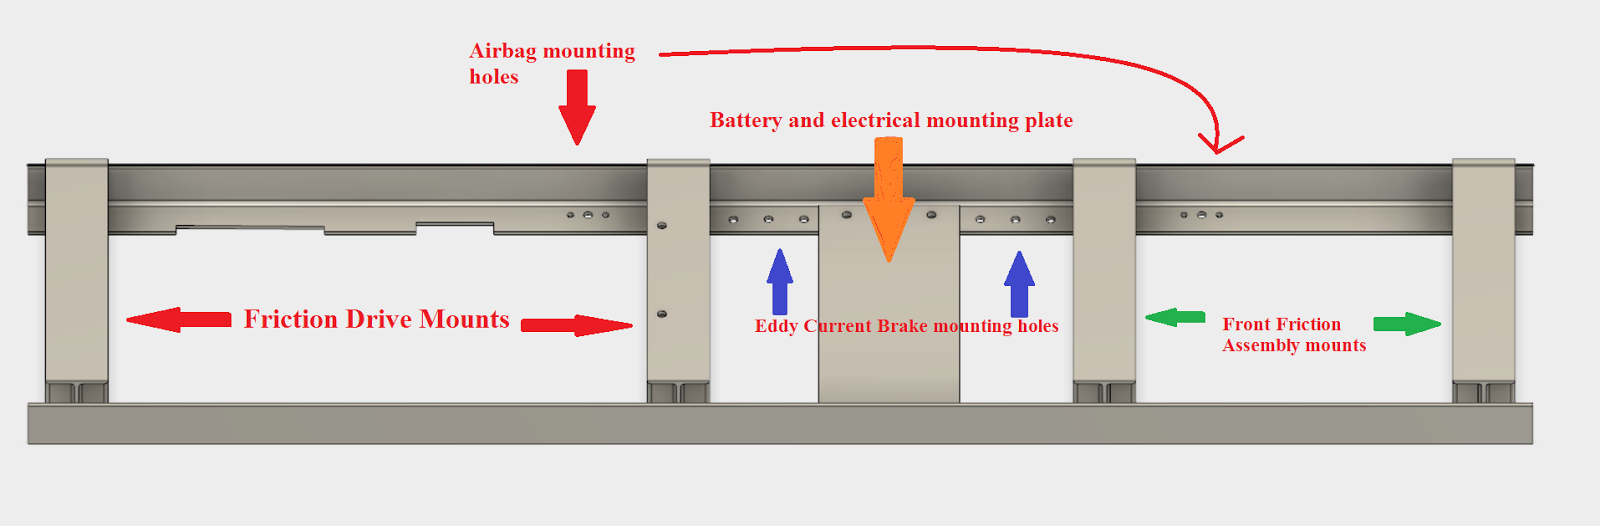
\includegraphics[width=\linewidth]{images/fig24}
        \caption{Caption needed}
    \end{figure}
    \begin{itemize}
        \item The mass of the whole frame will be approximately 25kg
        \item Dimensions would be 2.1m x 0.44m
    \end{itemize}
    Full cost breakdown, comments on manufacturability and production costs\\
    “A full Bill of Materials can be found in Appendix C.”
    
    \subsection{Structural}
    Modes of vibration (accounting for other subsystem masses)\\
    Dampening for those modes of vibration\\
    Speeds at which these modes of vibration can become a problem\\
    What are several reasonable and edge-case loading scenarios, and how does the FEA look for all of those? Justify your “reasonable” scenarios. If possible to simulate, how many cycles might it withstand?
    \begin{figure}[H]
        \centering
        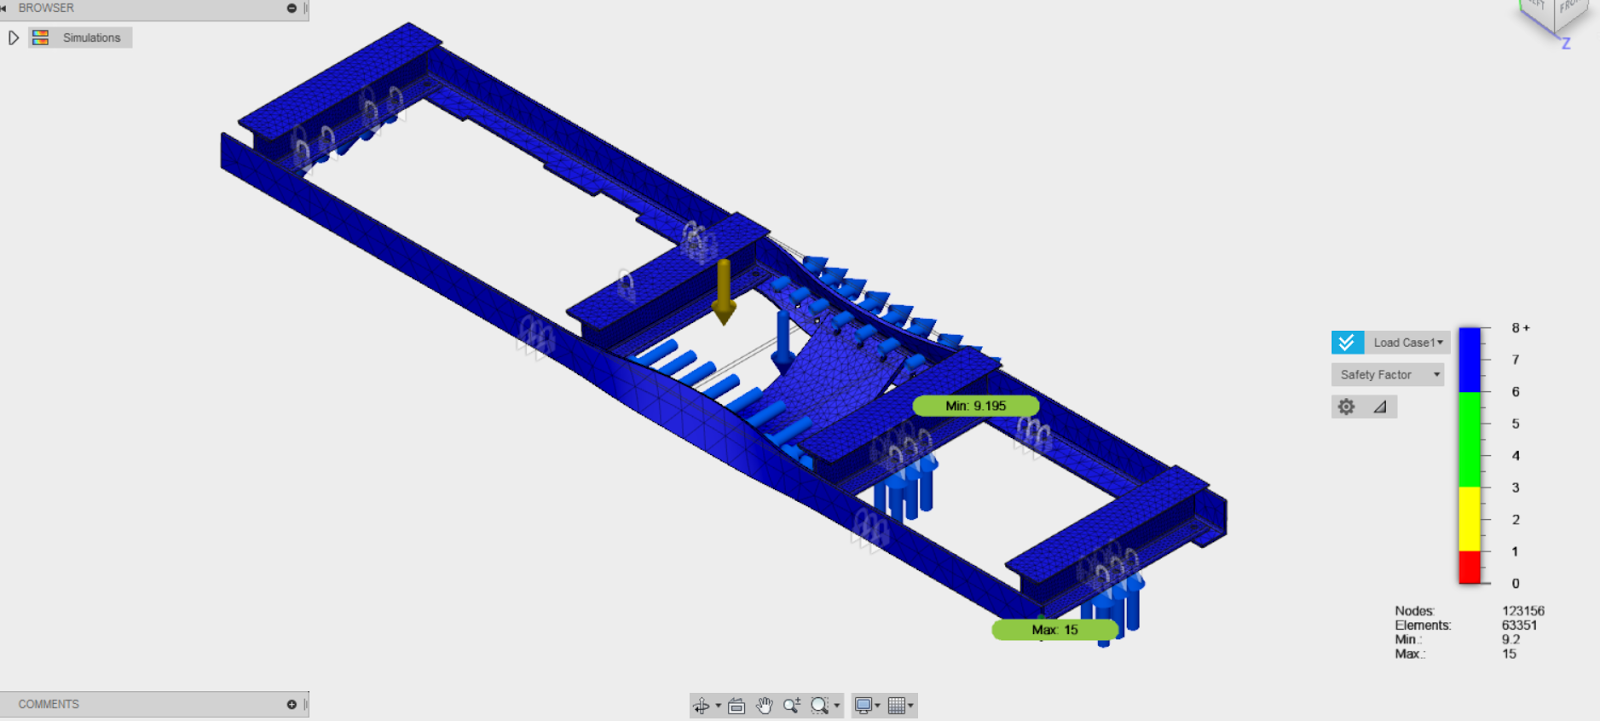
\includegraphics[width=\linewidth]{images/fig25}
        \caption{Caption needed}
    \end{figure}
    \begin{itemize}
        \item Profile if Braking was active, and friction drive was running
        \item Pod structural design cases: at a minimum, this shall include initial acceleration, nominal deceleration, and a reasonably foreseeable off-nominal crash (FEA)
    \end{itemize}
    
    \section{Shell}
    Justifications for design decisions
    \subsection{Overall Design}
    Full labeled detailed CAD\\
    Mass, dimensions, etc.\\
    Full cost breakdown, comments on manufacturability and production costs\\
    “A full Bill of Materials can be found in Appendix C.”
    
    \subsection{Aerodynamics}
    Analysis of aerodynamic coefficient\\
    Justification that this will not hit the Kantrowitz limit, and that the aerodynamic drag will be negligible
    
    \subsection{Structural}
    Choice of material - fiberglass vs carbon fibre\\
    What are several reasonable and edge-case loading scenarios, and how does the FEA look for all of those? Justify your “reasonable” scenarios. If possible to simulate, how many cycles might it withstand?\\
    Vacuum compatibility\\
    How do we deal with vibration?
    
    \section{Electrical}
    Mass, power consumption tables\\
    Fault tolerance, potential failure modes (FMEA)\\
    Whether it’s a single point of failure, and how to manage that\\
    Tests \& Validation (completed and planned)\\
    Cost breakdown\\
    Bill of Materials; whether it’s off the shelf or custom built.\\
    
    ABS Specs for 3D printing.\\
    Volume: \SI{0.80}{cm^3/g} or \SI{800}{cm^3/kg}.\\
    \SI{1.75}{mm} filament length per \SI{1}{kg} spool: $\sim \SI{330}{m}\ / \sim \SI{1080}{ft}$\\
    ABS. Cost: $\$\SI{30}{/kg} \rightarrow \$\SI{0.03}{/g}$\\
    
    Connectors\\
    
    Copper Wiring\\
    
    
    
    
    Safety and handling\\
    Ilya’s doc + modification\\
    Detailed CAD, as well as a picture of where it is in the main CAD.\\
    Justin will provide cads. \\
    Manufacturability; current build status if applicable\\
    Wire Management\\
    Insulation and harnessing\\
    Connectors\\
    Mass \\
    Materials (ABS, Aluminium, Copper)\\
    
    
    University of Waterloo has spot welding equipment for connecting cells in series.
    3D print cell supports using ABS plastic. E5 print room has 3D printers for that purpose.
    Graphs and visuals\\
    
    Justifications for design decisions - including selection process for design candidates and OTS products.\\
    
    Vacuum compatibility\\
    
    \subsection{Battery}
    \subsubsection{Design Criteria}
    \subsubsection{535V Battery}
    The 535V battery will be referred to as the main battery for the rest of this document.\\
    
    \begin{table}[H]
        \centering
        \begin{tabular}{@{}lr@{}} \toprule
            Specification & Emrax 268 motor\\ \midrule
            Peak Voltage & \SI{680}{V}\\
            Operating Voltage & \SI{400}{V}\\
            RPM per Volt & \SI{7.5}{rpm} (estimated)\\
            Torque per Amp & \SI{1.4}{Nm}\\
            Power (peak) & \SI{230}{KW}\\
            Power (continuous) & \SI{100}{KW}\\
            Torque (peak) & \SI{500}{Nm}\\
            Torque (continuous) & \SI{250}{Nm}\\ \bottomrule
        \end{tabular}
        \caption{Motor Specifications}
    \end{table}
    
    \begin{table}[H]
        \centering
        \begin{tabular}{@{}lr@{}} \toprule
            Specification & Main Battery\\ \midrule
            Max Voltage & \SI{535}{V}\\
            Peak Current & \SI{337.5}{A}\\
            Power (peak) & \SI{135}{KW}\\
            Power (continuous) & \SI{97.5}{KW}\\ \bottomrule
        \end{tabular}
        \caption{Main Battery Specifications}
    \end{table}
    This battery will power the motor and will be assembled with LiPo cells from HobbyKing. HobbyKing is a manufacturer that tailors to RC hobby planes, which draw high current for short bursts of time, which is a relatively similar use case to the Goose 3.  Furthermore, they are readily accessible in low quantities such that the team can place rush orders if necessary.  Many other cell chemistries and other Lithium Polymer cells were considered, however the Nanotech batteries (with specs stated above) were chosen for their low cost, high discharge rate, and similar intended use case. The BMS is being outsourced to Elithion, who has a reputation for building reliable Battery Management Systems for many different prototypes and student design teams. Factors such as internal resistance have been factored into the determination of the battery voltage. As seen in the table above, in order to achieve desired speed, the battery voltage must not drop below 385 V.  Thus, a conservative value of 400V was decided as the minimum expected voltage of the battery within it’s approximately 11 second run. Running at \SI{67}{\celsius}, this means the maximum voltage of the battery must be approximately 550 V.
    \begin{itemize}
        \item 4.2V(peak), 3.7V (nominal), 3700mAh, 337.5A (90C)
        \item Design of cell/module/battery. Include dimensions of each.
        650V battery power consumption table
    \end{itemize}
    Screenshots of CAD models
    \begin{itemize}
        \item Cell terminals to be spot welded in series. 4/5 cells in each module. Want to use entire surface of terminal.
        \item 32 modules connected in series.??
        \item BMS only has input for 16 modules, so will need to connect two modules together to meet the maximum number of input. 
    \end{itemize}
    \subsubsection{24V Battery}
    \begin{table}[H]
        \centering
        \begin{tabular}{@{}lrc@{}} \toprule
            Specification & Main Battery & Unit\\ \midrule
            Maximum Voltage & 25.2 & \si{V}\\
            Nominal Voltage & 22.2 & \si{V}\\
            Minimum Voltage & 19.2 & \si{V}\\
            Capacity & 7.5 & \si{Ah}\\
            Current Draw & 3.06 & \si{A}\\
            Power Draw & 40 & \si{W}\\
            Discharge Rate & 0.41 & \si{C}\\
            Time to Discharge & 2.45 & \si{h}\\ \bottomrule
        \end{tabular}
        \caption{24V Battery Specifications}
    \end{table}
    The 24V battery will be constructed of the same cells as the main battery. This decision was made to be resource and cost efficient, since designs and materials from the main battery can be carried over.. The battery will be contained within the same housing as the main battery. The cell arrangement is 6S2P, and will be built from the same cells as the main battery.The 24V battery will power the embedded system, including all sensors (including ESC’s additional functions). In the instance the 24V battery fails, there will be a backup battery with identical specs, but with half the capacity (6S1P configuration). This backup battery will be held isolated from the other batteries in  a location identified in the sensor map (in embedded section). This location was chosen due to the short distance from friction and EC brakes, which would need to be activated in case of an emergency.
    \begin{table}[H]
        \centering
        \begin{tabular}{@{}lrrrrrc@{}} \toprule
            Component & Quantity & \makecell{Operating \\ Voltage (V)} & \makecell{Current \\ Draw/Unit (A)} & \makecell{Total Current \\ Draw (A)} & \makecell{Power \\ Draw (W)} & Notes\\ \midrule
            Arduino Nano & 6 & 5 & 0.0334 & 0.2004 & 1.002 &\\
            Arduino Mega & 3 & 5 & 0.05 & 0.15 & 0.75 &\\
            Raspberry Pi & 2 & 5 & 0.7 & 1.4 & 7 &\\
            Contact Temp. & 8 & 5 & 0.00005 & 0.0004 & 0.002 &\\
            IR Temp & 8 & 3.3 & 0.00024 & 0.00192 & 0.006336 &\\
            PED & 4 & 24 & 0.1 & 0.4 & 9.6 &\\
            IMU & 2 & 3.3 & 0.0016 & 0.0032 & 0.01056 &\\
            ESC & 1 & 24 & 0.9 & 0.9 & 21.6 & \makecell{Inrush \\ current of 4A}\\ \midrule
            Total & & & & 3.05592 & 39.970896 &\\ \bottomrule
        \end{tabular}
        \caption{Consumption of Components}
    \end{table}
    \paragraph{Wire Management}
    The wire used to power the motor needs to support a voltage of 625V and a current of 205A. This will need to run from the battery to the motor, which are about 0.5m apart from each other. According to guidelines outlined by Blue Sea Systems Inc.\footnote{“Part 1: Choosing the Correct Wire Size for a DC Circuit.” Internet: https://www.bluesea.com/resources/1437, May 19, 2010 [Dec 17, 2017]}, this wire needs to be a 2|0 AWG copper wire. The arduinos and sensors do not require a current greater than 5A, so they can use 16 AWG copper wire.\\
    
    Wires will be routed such that power lines for main battery will be as far away as possible from all other cables (to avoid interference).
    
    \begin{itemize}
        \item Add notes above harness, connectors (cannon and molex microfit jr.) connections intended to be used
    \end{itemize}
    
    \subsubsection{Battery Management System}
    \paragraph{Main Battery}
    \begin{itemize}
        \item BMS
    \end{itemize}
    
    \paragraph{24V Battery}
    The 24V battery will use a commercially available 6S BMS. In order to ensure the BMS works as advertised, very basic tests will be conducted (i.e. try to draw current above what BMS is restricted to).
    \subsubsection{Battery Charging}
    \paragraph{Main Battery}
    \begin{itemize}
        \item Charging
    \end{itemize}
    \paragraph{24V Battery}
    The 24V battery will be charged through standard hobbyist grade LiPo cell chargers, which are already owned by the team.\\
    
    ESC, how power will be transferred and ensured for safety
    
    \subsection{Circuit Diagrams \& Flowcharts}
    \begin{itemize}
        \item Safety Circuits
    \end{itemize}
    \subsection{Failsafes}
    \begin{itemize}
        \item Main power loss immediately activates EC brakes and disables motors.
        \item Software power loss does the same thing.
    \end{itemize}
    \begin{table}[H]
        \centering
        \begin{tabular}{@{}lll@{}} \toprule
            & Operational & Failed\\ \midrule
            EC Brakes & Normally open \& Brakes disengaged & Go to Normally Closed \& Brakes engage\\
            Friction Brakes & Friction brake disengaged & If speed is below \_ m/s, engage friction brakes.\\
            IMU & \makecell[l]{Powered by Arduino 3.3V line (which \\ will be powered via 24V battery).} & \makecell[l]{IMU (and associated Arduino) will be \\ powered via backup LiPo cell.}\\
            Discharge Circuit & Not operational & \makecell[l]{Discharge battery through a capacitor and \\ power resistor.}\\ \bottomrule
        \end{tabular}
        \caption{Caption}
    \end{table}
    Hardware and software inhibits on braking during the acceleration phase
    \begin{itemize}
        \item E.g. electrically cut power to the motor if brakes engage
    \end{itemize}
    \subsection{Thermal}
    \subsection{Testing}
    Since different cell chemistries (even similar ones) react differently to various incidents (i.e. puncturing the cell), it was determined that the most effective way to show the battery design will be safe would be to experimentally test various components of the batteries to varying  extents, and using experimentally derived results to determine safe operating ranges for the batteries. The 3.7 V batteries used as backup power for the Arduino and Raspberry Pi have already been tested previously by our team in a vacuum, drawing expected current draw with no issues. Outlined below are general testing plans for the main and 24V battery. They will be furthered expanded upon once details of testing have been finalized.
    \subsubsection{Purpose of Testing}
    To determine the absolute limits of batteries and to determine expected range of values for battery including temperature, current, and voltage under various different conditions.
    \subsubsection{Parameters of Testing}
    All cell level testing (testing levels will be described later further on) will be done to failure with the exception of vacuum testing (in order to protect testing equipment). With the exception of vibration testing, module level testing will be tested to failure with the exception of vibration testing, which will be done through a wide range of frequencies. The final battery will undergo no destructive testing however testing from all level testings should provide a thorough analysis of how final battery will react to various different unexpected scenarios.
    \subsubsection{Equipment for Testing}
    Temperature sensors (both IR and contactless) will be used to monitor temperature of batteries in all tests. A shunt resistor and arduino will be used to measure current and voltage at all times, in all tests. Impact testing and hydraulic press testing will most likely be performed at university facilities, however facilities have not been confirmed. Vibration testing will be performed at Infinity Testing Solutions, however use of facilities for Goose III have not been confirmed.
    \subsubsection{Testing Procedure}
    Side Note: Testing will be broken into three “levels”; cell testing, module testing and battery testing. This testing is specifically with regards to the 535V battery. While the other batteries (24V and 3.7 V) will be tested, the 535V battery will be tested to the most rigorous degree, as a failure of this battery would lead to a significantly more catastrophic outcome than the other ones.
    
    \paragraph{Level One: Cell Testing}
    This level of testing is where the most destructive testing will occur, since cells are relatively cheap in comparison to modules and the full battery. The cells being tested on will be from the Turnigy’s Nano-tech Ultimate  7500 mAh 2S2P. Since the battery comes in a variety of different capacities, all cell level testing will be done on both the 3750 mAh cells as well as the 1300 mAh cells, to determine the consistency of the specific cell chemistry. This will help the team, in the instance our power demands change and a change in capacity is required. The cell level tests include:
    \begin{enumerate}
        \item \textbf{Mechanical Damage}
        \begin{enumerate}
            \item \textit{Impact Testing}
            \begin{enumerate}
                \item \textbf{What: }Use impact testing facilities to expose the cells to impulses of increasing values, until failure.
                \item \textbf{Why: }To understand what precautions need to be taken while transporting the batteries, whether this is driving the battery to competition, what to expect if the battery is accidentally dropped, and any other potential cases that may damage the battery.
                \item \textbf{Recorded Data: }Qualitative analysis (including video) and maximum impulse a cell can handle from various angles.
                \item \textbf{Next steps: }To model the full battery based on the results from cell testing.
            \end{enumerate}
            \item \textit{Puncture Testing}
            \begin{enumerate}
                \item \textbf{What: }Use a nail to puncture the cells in various locations.
                \item \textbf{Why: }To understand what will happen if cell is accidentally punctured during assembly or transport.
                \item \textbf{Recorded Data: }Qualitative analysis (including video) and heat generated over time.
                \item \textbf{Next Steps: }N/A
            \end{enumerate}
        \end{enumerate}
        \item \textbf{Over Current Damage}
        \begin{enumerate}
            \item \textbf{What: }Short the two leads of the battery together in a safe environment.
            \item \textbf{Why: }To understand what will occur in case of a short, since various LiPo cells  react differently when shorting (some, just gas, while others start a fire).
            \item \textbf{Recorded Data: }Qualitative analysis (including video), maximum dimensions of cell (via video analysis) and heat generated.
            \item \textbf{Next Steps: }Model the full battery overcurrent damage based on data from cell damage.
        \end{enumerate}
        \item \textbf{Over Charging Damage}
        \begin{enumerate}
            \item \textbf{What: }Charge cell to increasing levels of voltage above 4.2 V max charge rating.
            \item \textbf{Why: }To test the maximum manufacturer rating for the battery, and to see how far above it the battery can go (or if it is even capable of reaching 4.2 V). Batteries used in competition will not be charged about maximum manufacturer rating nor will they have been previously charged above this value. The overcharge component of the test is purely for testing purposes.
        \end{enumerate}
        \item \textbf{Cycle Testing}
        \begin{enumerate}
            \item \textbf{What: }Cycle cells at various discharge rates, including and above our expected discharge rate.
            \item \textbf{Why: }To determine the expected life cycle of the full battery. If our battery is used for different purposes in the future, expected lifespan can then be calculated from tests at different discharge rates. Furthermore, this will help determine whether or not the battery manufacturer’s listed specs are valid.
            \item \textbf{Recorded Data: }Qualitative analysis (including video), cell charge and discharge rates and times, charge capacity, heat generation, and cell initial and final dimensions (plus any other notable dimension changes if any).
            \item \textbf{Next Steps: }N/A
        \end{enumerate}
        \item \textbf{Vacuum Testing}
        \begin{enumerate}
            \item \textbf{What: }High current testing in a vacuum up to 90C or until it appears (both qualitatively and thermally) the cell is about to explode. This test must be conducted last of the five cell level tests. While the order of other tests does not matter, this test must be conducted last. The data of the other tests will provide expected ranges in which the battery can safely operate (i.e. temperature, expansion, etc.). There must be automatic shutoffs in place when any value exceeds safe ranges in order to avoid damaging the testing facility.
            \item \textbf{Why: }To ensure the battery will operate safely in a vacuum, while drawing a high current, since pressure changes may cause increase expansion rate.
            \item \textbf{Recorded Data: }Qualitative analysis (including video), current and voltage draw,
            \item \textbf{Next Steps: }If cells do expand due to testing, determine whether or not the cells can be safely used in the design, or if new cell needs to be used
        \end{enumerate}
    \end{enumerate}
    \paragraph{Level Two: Module Testing}
    This level of testing will be conducted on modules (4S). The cells being tested on will be from the Turnigy’s Nano-tech Ultimate  7500 mAh 2S2P. Since the battery comes in a variety of different capacity’s, all cell level testing will be done on both the 3750 mAh cells as well as the 1300 mAh cells (if time and budget permits), to determine the consistency of the specific cell chemistry. This will help the team, in the instance our power demands change and a change in capacity is required. The module level tests include:
    \begin{enumerate}
        \item \textbf{Expansion Testing}
        \begin{enumerate}
            \item \textbf{What: }Allow x number of cells (where x ranges from 1-4) to expand via a short circuit.
            \item \textbf{Why: }To determine what will happen in the instance a cell (or multiple cells) within a module expand.
            \item \textbf{Recorded Data: }Qualitative analysis (including video), and thermal analysis.
            \item \textbf{Next Steps: }Design and test multiple different module enclosures, to determine the safest, effective design.
        \end{enumerate}
    \end{enumerate}
    \paragraph{Level Three: Full Battery Testing}
    This level of testing will be conducted with the full battery (650V), in its completed arrangement. There will be no destructive testing at this level (due to cost), and data provided from previous tests should set parameters at which the battery can safely operate. The data from this level of testing should correlate with results from previous tests, however the current draw will be incrementally increased to avoid damage from unexpected factors. The first two tests will be conducted with a large number of temperature sensors (and potentially a thermographic camera) to create a simulated “map” of the battery’s temperature at any given location. From there the 3-4 points that have the tendency to be the hottest will chosen for the final sensor setup. The latter two tests will only use this 3-4 points of temperature monitoring, and will be conducted at competition using SpaceX’s vacuum facilities.
    \begin{enumerate}
        \item \textbf{Motor No Load Testing}
        \begin{enumerate}
            \item \textbf{What: }Incrementally increasing current draw from motor, until at max expected draw of 55C.
            \item \textbf{Why: }To ensure the motor, BMS, and ESC all work in conjunction with one another.
            \item \textbf{Recorded Data: }Qualitative analysis (including video), thermal profile, RPM of motor, and any other info the ESC and BMS will provide.
            \item \textbf{Next Steps: }N/A
        \end{enumerate}
        \item \textbf{Motor With Load Testing}
        \begin{enumerate}
            \item \textbf{What: }Once friction drive has been assembled and both the friction drive and battery have been integrated, the same test as the previous test will be conducted. If there is a test track available, there will be a second component to this test in which the pod will move down the racetrack.
            \item \textbf{Why: }To ensure the friction drive has been assembled correctly, and will function as expected.
            \item \textbf{Recorded Data: }Qualitative analysis (including video), and all sensor info from embedded system.
            \item \textbf{Next Steps: }N/A
        \end{enumerate}
        \item \textbf{Vacuum Testing}
        \begin{enumerate}
            \item \textbf{What: }Test the battery (with electronics powered on) within SpaceX’s vacuum testing facility.
            \item \textbf{Why: }To ensure everything works as expected.
            \item \textbf{Recorded Data: }Data from embedded systems.
            \item \textbf{Next Steps: }N/A
        \end{enumerate}
        \item \textbf{Motor Testing in Vacuum}
        \begin{enumerate}
            \item \textbf{What: }Test the pod down SpaceX’s race track.
            \item \textbf{Why: }To ensure everything works as expected.
            \item \textbf{Recorded Data: }Data from embedded systems.
            \item \textbf{Next Steps: }N/A
        \end{enumerate}
    \end{enumerate}
    \paragraph{General Next Steps (this includes tests marked N/A)}
    An initial Battery Safety 101 will be conducted with all members who participate in testing. Furthermore, all results from level one and two testing will be incorporated into a secondary Battery Safety Training which provide all necessary info on what to do with a cell, module or battery in any given instance.Training will be given to all members involved in battery construction, as well as the Integration leads. If at any point of testing, the batteries are deemed to be “too dangerous” (i.e. vacuum testing shows that cells will burst when drawing expected discharge rate of 55C), the team must go back to the drawing board and determine a new potential cell candidate.
    \section{Embedded}
    \subsection{Microcontroller}
    \subsection{Custom Software}
    \subsection{Buses}
    \subsection{Main Embedded Board}
    Raspberry Pi’s will be socketed on the main embedded board face down (as described by the CAD). Due to the complexity of the board, and minimal space saved by integrating the board onto the main embedded system, the Pi will not be integrated directly onto the main embedded. Furthermore, in case of a malfunction it is more cost and time effective to replace a singular Pi instead of replacing the entire board. The Arduino Mega will be integrated directly onto the board. Since once complete the Arduinos will not have to be frequently updated, it would be efficient to simply use a ATmega 328, DIP-28 package and pop it out to program it on a regular Mega board when necessary. The choice for a DIP package over a TQFP was also made such that a blown chip would not lead to the entire board having to be replaced.
    
    \subsection{Subsystem Boards}
    Originally, the embedded team decided to use an Arduino Uno, with a CANBUS shield stacked on top, with a seperate board with the connections to the external connectors on it. However, most of the pins on both the arduino and the CANBUS were completely unnecessary. With said design, the embedded for a single subsystem would be almost triple the size of an Arduino Uno, with significantly more sources of error (the Arduino, the CANBUS, and a board housing connectors would have to be connected together).  Upon considering that there would have to be multiple of these housings, it was decided that all three boards could be integrated into a singular one, with the approximate size of an Arduino Uno. Once the final revision is designed, multiple copies of the same board will be printed and populated. For initially testing purposes however the original setup of an Uno with a CANBUS shield will be used, until the PCB is printed and thoroughly tested. 
    
    \subsection{Sensors}
    \subsubsection{Temperature}
    \subsubsection{Current}
    \subsubsection{Tilt}
    \subsubsection{Navigation}
    \subsubsection{Lateral Stability}
    \subsubsection{EC-Brake State}
    \subsubsection{Pressure}
    
    \subsection{Thermal}
    \subsection{Flowcharts}
    
    \subsection{Physical Hardware}
    Mass, power, etc.\\
    How will these things be powered? Mini lipo battery packs?\\
    How is it mounted? CAD? Does it need to be in a pressure chamber?\\
    Will the processors get very hot due to vacuum? How will they be cooled?\\
    Will the system have components susceptible to vacuum? (e.g. some capacitors) Briefly justify an answer of “no.” How will we test this?\\
    Rationale for choosing Raspberry Pi and Arduino\\
    Cost breakdown
    
    \subsection{Software System Structure}
    \subsubsection{Terminology}
    \begin{itemize}
        \item Control-Panel - UI interface running on a remote machine to visualize data and control pod
        \item Master Machine - RaspberryPi 3B computer running Waterloop’s communication-system
        \item Slave Machine - Arduino Due running Waterloop’s embedded-system
        \item CAN Data Packet - Custom binary packet type created by team Waterloop
    \end{itemize}
    \subsubsection{Design Criteria}
    The main goal when building the software systems around the pod was creating a redundant, yet lightweight and fast solution that would allow for safe communications with the vehicle and ensure control throughout pod launch. The Software-system is built upon the Master-Slave design model to allow for maximum redundancy and safety at all times. The design is based on three components: embedded systems (Slave), communication systems (Master), and control-panel. Embedded-systems is responsible for all of the pod’s internal interactions with the sensors and various health checks. Communication-systems is responsible for the complete pod control and has the ability to safely shut down the pod in case of an emergency. It is also responsible for the transportation of information from the vehicle to the front-end to allow for live data visualization and remote control of the pod. Front-end is responsible for displaying all of the pod’s vital readings and providing an interface to control the pod while in the tube. All of the code written for the software system of the pod is available for public access at Waterloop’s github page.
    \subsubsection{System Overview}
    Building off the model of Master-Slave design, Waterloop has defined two clear computational layers Master Machines and Slave Machines. Master machines are responsible for the complete control of the pod and the transfer of data from Slave Machines to the Control-Panel. Two main design decisions of the Goose III’s computational design are the parallelism of launch script execution and the Master-slave design.
    \begin{itemize}
        \item Having Master-Slave design in place, we can ensure the validity of data coming from the Slave Machines. When Slaves acquire data from sensors, there is a possibility of a slave providing errant data. To handle the case of an errant slave, Masters have the voting capability to compare the results of three slaves, detect the errant device and act appropriately
        \item With parallel execution by the two Master machines, in case of one of the machines coming offline for any unforeseen reason, the switch to the next machine is instantaneous
    \end{itemize}
    \textbf{[INSERT SOFTWARE DIAGRAM HERE]}\\
    Based on the software diagram above, the entire system will incorporate \textbf{[Number of sensors]} sensors and an ESC, that will allow for a complete control over the pod and a live stream of data from all sensors.
    \subsubsection{Control Packet Format}
    \paragraph{JSON}
    All communications between onboard computers and frontend controls are JSON packets serialized from Go structs in the following format:
    \begin{verbatim}
    type CommPacketJson struct {
    Time int64     `json:"time"`
    Type string    `json:"type"`
    Name string    `json:"name"`
    Data []float32 `json:"data"`
    }
    \end{verbatim}
    \begin{table}[H]
        \centering
        \begin{tabular}{@{}lll@{}} \toprule
            Property & Description & Example\\ \midrule
            \verb|time| & Time of packet creation, in milliseconds since Unix epoch & \verb|1513452619442|\\
            \verb|type| & Packet type, see possible packet types & \verb|"sensor"|\\
            \verb|name| & \makecell[l]{Specific name of packet, explicitly describing role and origin of packet \\ (i.e. data from a specific sensor)} & \verb|"accel1"|\\
            \verb|data| & 3-tuple of float32 values representing packet data & \verb|[32.2323, 12.22, 23.11]|\\ \bottomrule
        \end{tabular}
        \caption{Explanation of fields}
    \end{table}
    Example of a serialized JSON:
    \begin{verbatim}
    {
    "time": 1513452619442,
    "type": "sensor",
    "name": "accel",
    "data": [0.00, 0.00, 0.00]
    }
    \end{verbatim}
    \subsubsection{Communication Protocol}
    Commands, sensor data, and events are sent between data machines, controllers, and web servers, using 64-bit packets. Packets are memory-		efficient, fast to read and write, and reliable. Packets are checked with a CRC-8 checksum $(0$x$97 = x^8 + x^5 + x^3 + x^2 + 1)$.
    \begin{table}[H]
    	\centering
    	\begin{tabular}{@{}lccccc@{}} \toprule
            Segment & Type & Sensor ID & Data 1 & Data 2 & Data 3 \\ \midrule
            Bits & 3 & 7 & 18 & 18 & 18 \\ \bottomrule
        \end{tabular}
        \caption{Caption here}
    \end{table} 
    Each packet contains 3 bits representing packet type, 7 bits representing origin sensor or device ID, and three 18-bit data segments. These are 18-bit floats with 1 bit for sign, 5-bit exponent width, and 13-bit significand precision (12 explicitly stored), similar to IEEE 754 specifications.
	\begin{figure}[H]
        \centering
        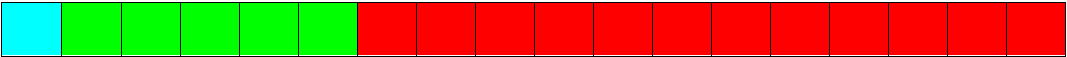
\includegraphics[width = \textwidth]{images/fig326.PNG}
    	\caption{Caption here}
    \end{figure}
    \subsection{Navigation System}
    \subsection{Library \& Build Infrastructure}
    We developed an in-house C++ library for use on microcontrollers (Arduino and Raspberry Pi). WLib is performant, memory efficient, has a small binary footprint, and is a safer alternative to STL. WLib uses a custom memory management solution with fixed-size memory pools, preventing fragmentation and leaks. It provides basic data structures (lists, sets, maps, trees), and smart pointers (shared and unique).
    \url{https://teamwaterloop.github.io/waterloop-wlib/}
    
    We also developed a custom Arduino build system and use Cosa, an object-oriented AVR platform, in place of the standard Arduino libraries. Cosa (\url{https://github.com/mikaelpatel/Cosa}) is faster and has lower power consumption.
    \subsection{Fault Tolerance \& Testing}
    \subsection{Pod Health}
    
    \chapter{Next Steps}
    
    \section{Manufacturing}
    \section{Tests}
    \subsection{Test Rigs}
    \subsection{Functional Tests}
    
    
    
    \chapter{References}
    
    \begin{appendices}
        \addtocontents{toc}{\protect\setcounter{tocdepth}{1}}
        \makeatletter
        \addtocontents{toc}{%
            \begingroup
            \let\protect\l@chapter\protect\l@section
            \let\protect\l@section\protect\l@subsection
        }
        \makeatother
        
        \chapter{Hazards \& FMEA}
        \chapter{Procedures}
        \chapter{Bill of Materials}
        \chapter{Part Drawings}
        \chapter{Engineering Calculations?}
        \chapter{Research Topics?}
        \addtocontents{toc}{\endgroup}
    \end{appendices}
    
    
\end{document}
